% Options for packages loaded elsewhere
\PassOptionsToPackage{unicode}{hyperref}
\PassOptionsToPackage{hyphens}{url}
%
\documentclass[
]{scrartcl}
\usepackage{lmodern}
\usepackage{amssymb,amsmath}
\usepackage{ifxetex,ifluatex}
\ifnum 0\ifxetex 1\fi\ifluatex 1\fi=0 % if pdftex
  \usepackage[T1]{fontenc}
  \usepackage[utf8]{inputenc}
  \usepackage{textcomp} % provide euro and other symbols
\else % if luatex or xetex
  \usepackage{unicode-math}
  \defaultfontfeatures{Scale=MatchLowercase}
  \defaultfontfeatures[\rmfamily]{Ligatures=TeX,Scale=1}
\fi
% Use upquote if available, for straight quotes in verbatim environments
\IfFileExists{upquote.sty}{\usepackage{upquote}}{}
\IfFileExists{microtype.sty}{% use microtype if available
  \usepackage[]{microtype}
  \UseMicrotypeSet[protrusion]{basicmath} % disable protrusion for tt fonts
}{}
\makeatletter
\@ifundefined{KOMAClassName}{% if non-KOMA class
  \IfFileExists{parskip.sty}{%
    \usepackage{parskip}
  }{% else
    \setlength{\parindent}{0pt}
    \setlength{\parskip}{6pt plus 2pt minus 1pt}}
}{% if KOMA class
  \KOMAoptions{parskip=half}}
\makeatother
\usepackage{xcolor}
\IfFileExists{xurl.sty}{\usepackage{xurl}}{} % add URL line breaks if available
\IfFileExists{bookmark.sty}{\usepackage{bookmark}}{\usepackage{hyperref}}
\hypersetup{
  pdftitle={Supplementary Material for: A Rough Guide to Pre-processing High-Frequency Animal Tracking Data},
  pdfauthor={Pratik R. Gupte; Christine E. Beardsworth; Orr Spiegel; Emmanuel Lourie; Allert I. Bijleveld},
  hidelinks,
  pdfcreator={LaTeX via pandoc}}
\urlstyle{same} % disable monospaced font for URLs
\usepackage[left=4cm, right=3cm, top=2.5cm, bottom=2.5cm]{geometry}
\usepackage{color}
\usepackage{fancyvrb}
\newcommand{\VerbBar}{|}
\newcommand{\VERB}{\Verb[commandchars=\\\{\}]}
\DefineVerbatimEnvironment{Highlighting}{Verbatim}{commandchars=\\\{\}}
% Add ',fontsize=\small' for more characters per line
\newenvironment{Shaded}{}{}
\newcommand{\AlertTok}[1]{\textcolor[rgb]{1.00,0.00,0.00}{\textbf{#1}}}
\newcommand{\AnnotationTok}[1]{\textcolor[rgb]{0.38,0.63,0.69}{\textbf{\textit{#1}}}}
\newcommand{\AttributeTok}[1]{\textcolor[rgb]{0.49,0.56,0.16}{#1}}
\newcommand{\BaseNTok}[1]{\textcolor[rgb]{0.25,0.63,0.44}{#1}}
\newcommand{\BuiltInTok}[1]{#1}
\newcommand{\CharTok}[1]{\textcolor[rgb]{0.25,0.44,0.63}{#1}}
\newcommand{\CommentTok}[1]{\textcolor[rgb]{0.38,0.63,0.69}{\textit{#1}}}
\newcommand{\CommentVarTok}[1]{\textcolor[rgb]{0.38,0.63,0.69}{\textbf{\textit{#1}}}}
\newcommand{\ConstantTok}[1]{\textcolor[rgb]{0.53,0.00,0.00}{#1}}
\newcommand{\ControlFlowTok}[1]{\textcolor[rgb]{0.00,0.44,0.13}{\textbf{#1}}}
\newcommand{\DataTypeTok}[1]{\textcolor[rgb]{0.56,0.13,0.00}{#1}}
\newcommand{\DecValTok}[1]{\textcolor[rgb]{0.25,0.63,0.44}{#1}}
\newcommand{\DocumentationTok}[1]{\textcolor[rgb]{0.73,0.13,0.13}{\textit{#1}}}
\newcommand{\ErrorTok}[1]{\textcolor[rgb]{1.00,0.00,0.00}{\textbf{#1}}}
\newcommand{\ExtensionTok}[1]{#1}
\newcommand{\FloatTok}[1]{\textcolor[rgb]{0.25,0.63,0.44}{#1}}
\newcommand{\FunctionTok}[1]{\textcolor[rgb]{0.02,0.16,0.49}{#1}}
\newcommand{\ImportTok}[1]{#1}
\newcommand{\InformationTok}[1]{\textcolor[rgb]{0.38,0.63,0.69}{\textbf{\textit{#1}}}}
\newcommand{\KeywordTok}[1]{\textcolor[rgb]{0.00,0.44,0.13}{\textbf{#1}}}
\newcommand{\NormalTok}[1]{#1}
\newcommand{\OperatorTok}[1]{\textcolor[rgb]{0.40,0.40,0.40}{#1}}
\newcommand{\OtherTok}[1]{\textcolor[rgb]{0.00,0.44,0.13}{#1}}
\newcommand{\PreprocessorTok}[1]{\textcolor[rgb]{0.74,0.48,0.00}{#1}}
\newcommand{\RegionMarkerTok}[1]{#1}
\newcommand{\SpecialCharTok}[1]{\textcolor[rgb]{0.25,0.44,0.63}{#1}}
\newcommand{\SpecialStringTok}[1]{\textcolor[rgb]{0.73,0.40,0.53}{#1}}
\newcommand{\StringTok}[1]{\textcolor[rgb]{0.25,0.44,0.63}{#1}}
\newcommand{\VariableTok}[1]{\textcolor[rgb]{0.10,0.09,0.49}{#1}}
\newcommand{\VerbatimStringTok}[1]{\textcolor[rgb]{0.25,0.44,0.63}{#1}}
\newcommand{\WarningTok}[1]{\textcolor[rgb]{0.38,0.63,0.69}{\textbf{\textit{#1}}}}
\usepackage{longtable,booktabs}
% Correct order of tables after \paragraph or \subparagraph
\usepackage{etoolbox}
\makeatletter
\patchcmd\longtable{\par}{\if@noskipsec\mbox{}\fi\par}{}{}
\makeatother
% Allow footnotes in longtable head/foot
\IfFileExists{footnotehyper.sty}{\usepackage{footnotehyper}}{\usepackage{footnote}}
\makesavenoteenv{longtable}
\usepackage{graphicx}
\makeatletter
\def\maxwidth{\ifdim\Gin@nat@width>\linewidth\linewidth\else\Gin@nat@width\fi}
\def\maxheight{\ifdim\Gin@nat@height>\textheight\textheight\else\Gin@nat@height\fi}
\makeatother
% Scale images if necessary, so that they will not overflow the page
% margins by default, and it is still possible to overwrite the defaults
% using explicit options in \includegraphics[width, height, ...]{}
\setkeys{Gin}{width=\maxwidth,height=\maxheight,keepaspectratio}
% Set default figure placement to htbp
\makeatletter
\def\fps@figure{htbp}
\makeatother
\setlength{\emergencystretch}{3em} % prevent overfull lines
\providecommand{\tightlist}{%
  \setlength{\itemsep}{0pt}\setlength{\parskip}{0pt}}
\setcounter{secnumdepth}{2}

\usepackage{fontspec}
% use nice fonts if available else use boring defaults

\usepackage{lineno}
\setmainfont{Times New Roman}
\setsansfont{Arial}

\linenumbers
\newlength{\cslhangindent}
\setlength{\cslhangindent}{1.5em}
\newenvironment{cslreferences}%
  {\setlength{\parindent}{0pt}%
  \everypar{\setlength{\hangindent}{\cslhangindent}}\ignorespaces}%
  {\par}

\title{Supplementary Material for: A Rough Guide to Pre-processing High-Frequency Animal Tracking Data}
\author{Pratik R. Gupte \and Christine E. Beardsworth \and Orr Spiegel \and Emmanuel Lourie \and Allert I. Bijleveld}
\date{2020-11-23}

\begin{document}
\maketitle

{
\setcounter{tocdepth}{2}
\tableofcontents
}
\hypertarget{processing-calibration-data}{%
\section{Processing calibration data}\label{processing-calibration-data}}

Here we show how the residence patch method (Barraquand and Benhamou \protect\hyperlink{ref-barraquand2008}{2008}; Bijleveld et al. \protect\hyperlink{ref-bijleveld2016}{2016}; Oudman et al. \protect\hyperlink{ref-oudman2018}{2018}) accurately estimates the duration of known stops in a track collected as part of a calibration exercise in the Wadden Sea.

\hypertarget{prepare-libraries}{%
\subsection{Prepare libraries}\label{prepare-libraries}}

First we prepare the libraries we need. Libraries can be installed from CRAN if necessary.

\begin{Shaded}
\begin{Highlighting}[]
\CommentTok{\# load libs}
\KeywordTok{library}\NormalTok{(data.table)}
\KeywordTok{library}\NormalTok{(atlastools)}
\KeywordTok{library}\NormalTok{(ggplot2)}
\KeywordTok{library}\NormalTok{(patchwork)}

\CommentTok{\# prepare a palette}
\NormalTok{pal <{-}}\StringTok{ }\NormalTok{RColorBrewer}\OperatorTok{::}\KeywordTok{brewer.pal}\NormalTok{(}\DecValTok{4}\NormalTok{, }\StringTok{"Set1"}\NormalTok{)}
\end{Highlighting}
\end{Shaded}

\hypertarget{access-data-and-preliminary-visualisation}{%
\subsection{Access data and preliminary visualisation}\label{access-data-and-preliminary-visualisation}}

First we access the data from a local file using the \texttt{data.table} package (Dowle and Srinivasan \protect\hyperlink{ref-dowle2020}{2020}).
We then visualise the raw data.

\begin{Shaded}
\begin{Highlighting}[]
\CommentTok{\# read and plot example data}
\NormalTok{data <{-}}\StringTok{ }\KeywordTok{fread}\NormalTok{(}\StringTok{"data/atlas1060\_allTrials\_annotated.csv"}\NormalTok{)}
\NormalTok{data\_raw <{-}}\StringTok{ }\KeywordTok{copy}\NormalTok{(data)}
\end{Highlighting}
\end{Shaded}

\begin{figure}
\centering
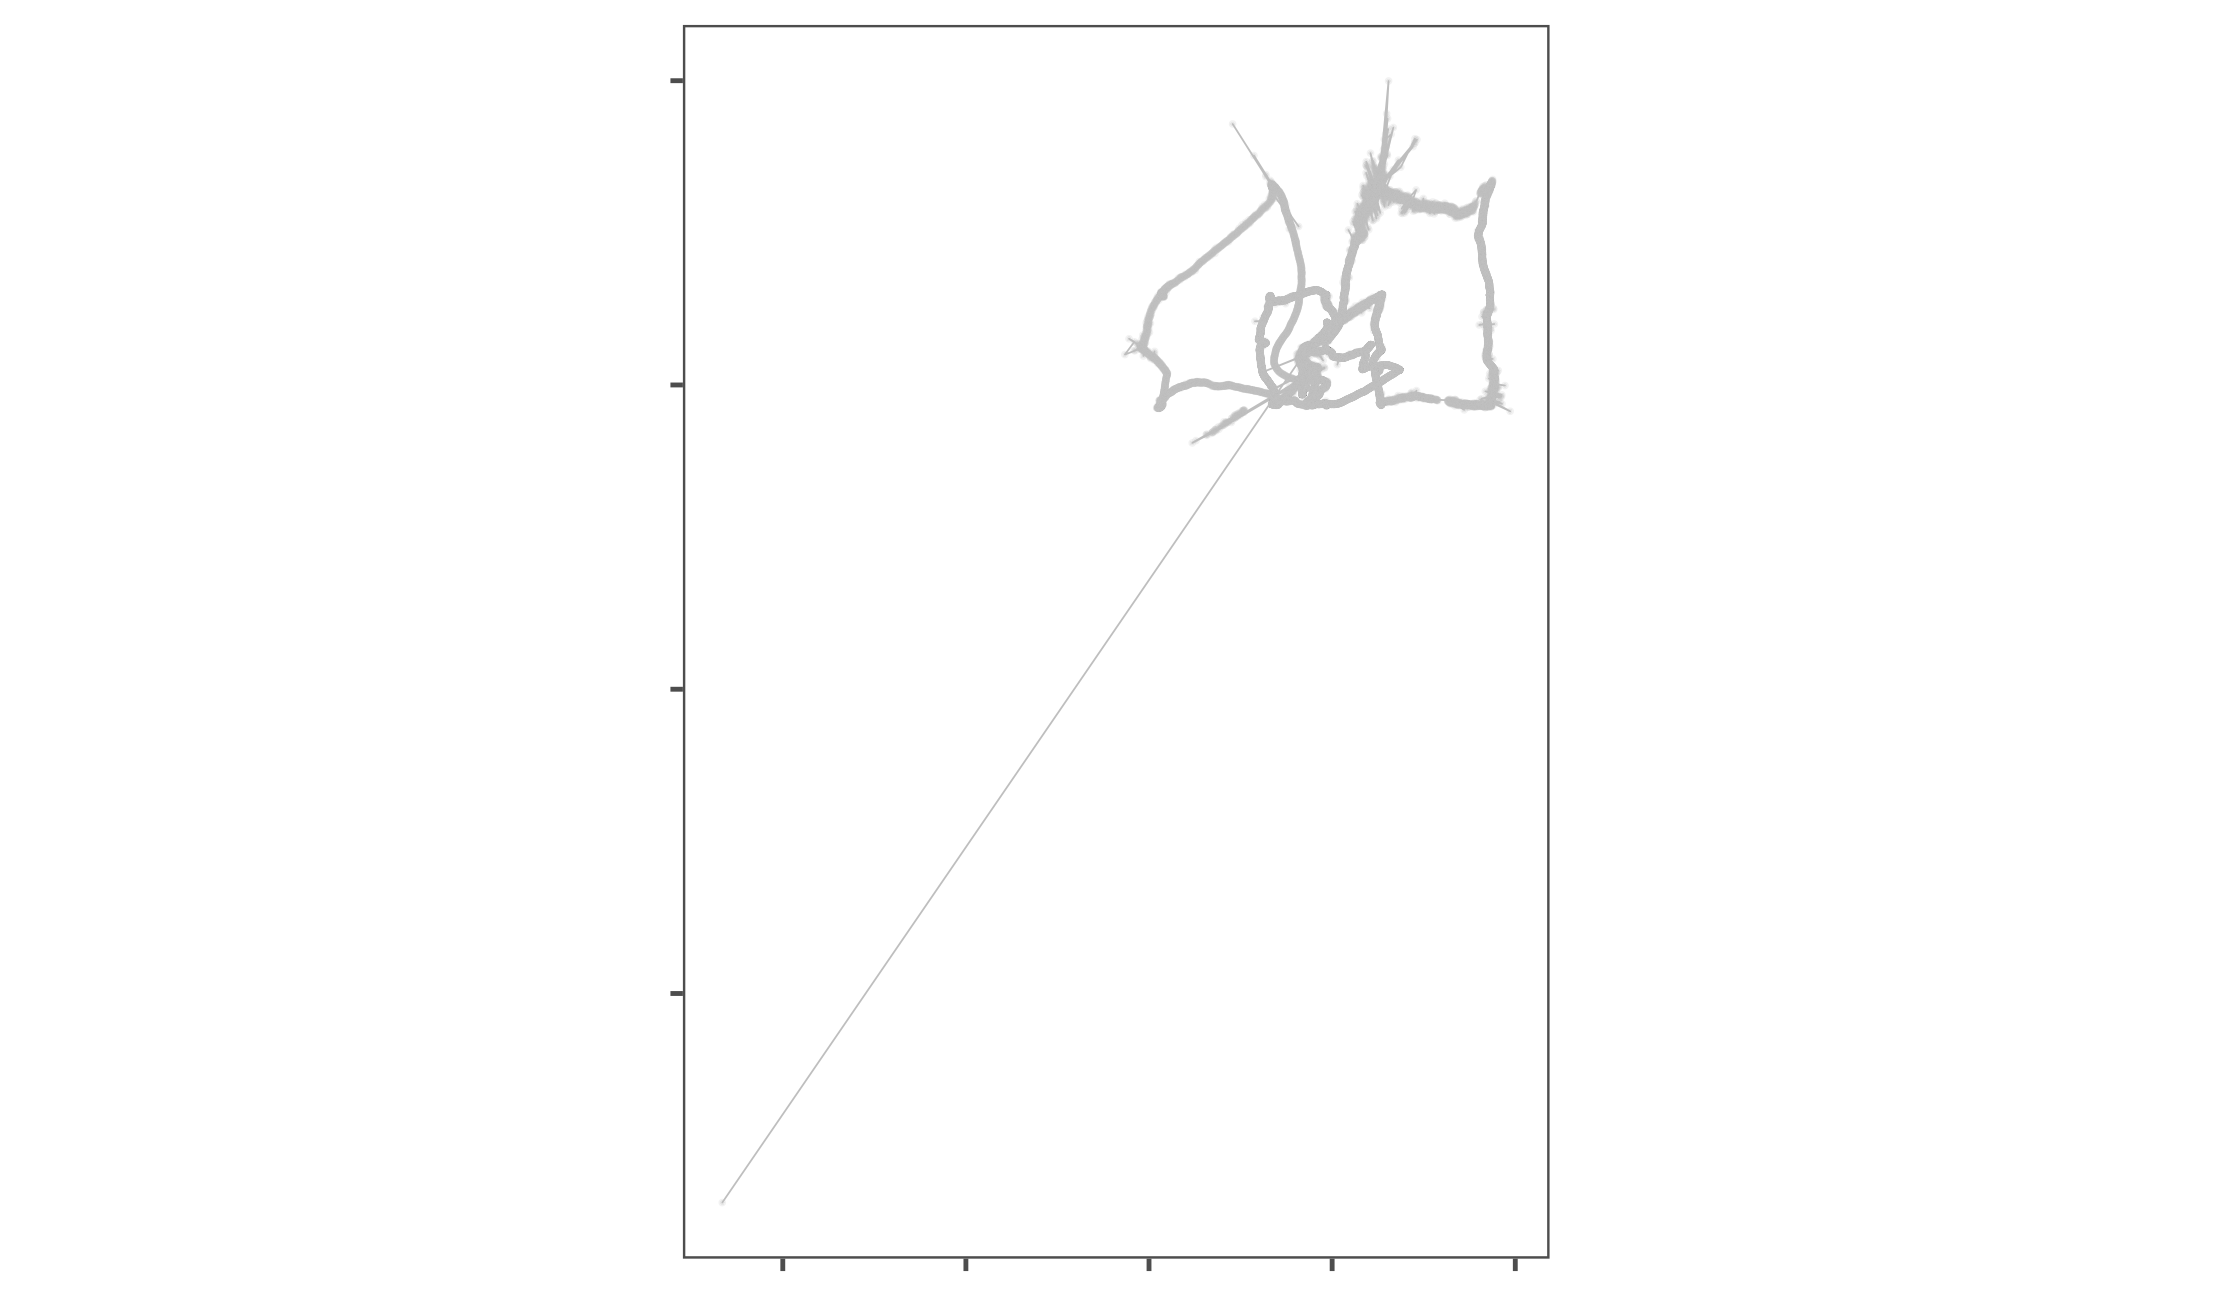
\includegraphics{figures/fig_calibration_raw.png}
\caption{The raw data from a calibration exercise conducted around the island of Griend in the Dutch Wadden Sea. A handheld WATLAS tag was used to examine how ATLAS data compared to GPS tracks, and we use the WATLAS data here to demonstrate the basics of the pre-processing pipeline, as well as validate the residence patch method. It is immediately clear from the figure that the track shows location errors, both in the form of point outliers as well as small-scale errors around the true location.}
\end{figure}

\hypertarget{filter-by-bounding-box}{%
\subsection{Filter by bounding box}\label{filter-by-bounding-box}}

We first save a copy of the data, so that we can plot the raw data with the cleaned data plotted over it for comparison.

\begin{Shaded}
\begin{Highlighting}[]
\CommentTok{\# make a copy using the data.table copy function}
\NormalTok{data\_unproc <{-}}\StringTok{ }\KeywordTok{copy}\NormalTok{(data)}
\end{Highlighting}
\end{Shaded}

We then filter by a bounding box in order to remove the point outlier to the far south east of the main track. We use the \texttt{atl\_filter\_bounds} functions using the \texttt{x\_range} argument, to which we pass the limit in the UTM 31N coordinate reference system.
This limit is used to exclude all points with an X coordinate \textless{} 645,000.

We then plot the result of filtering, with the excluded point in black, and the points that are retained in green.

\begin{Shaded}
\begin{Highlighting}[]
\CommentTok{\# remove inside must be set to falses}
\NormalTok{data <{-}}\StringTok{ }\KeywordTok{atl\_filter\_bounds}\NormalTok{(}\DataTypeTok{data =}\NormalTok{ data, }
                          \DataTypeTok{x =} \StringTok{"x"}\NormalTok{, }\DataTypeTok{y =} \StringTok{"y"}\NormalTok{, }
                          \DataTypeTok{x\_range =} \KeywordTok{c}\NormalTok{(}\DecValTok{645000}\NormalTok{, }\KeywordTok{max}\NormalTok{(data}\OperatorTok{$}\NormalTok{x)), }
                          \DataTypeTok{remove\_inside =} \OtherTok{FALSE}\NormalTok{)}
\end{Highlighting}
\end{Shaded}

\begin{figure}
\centering
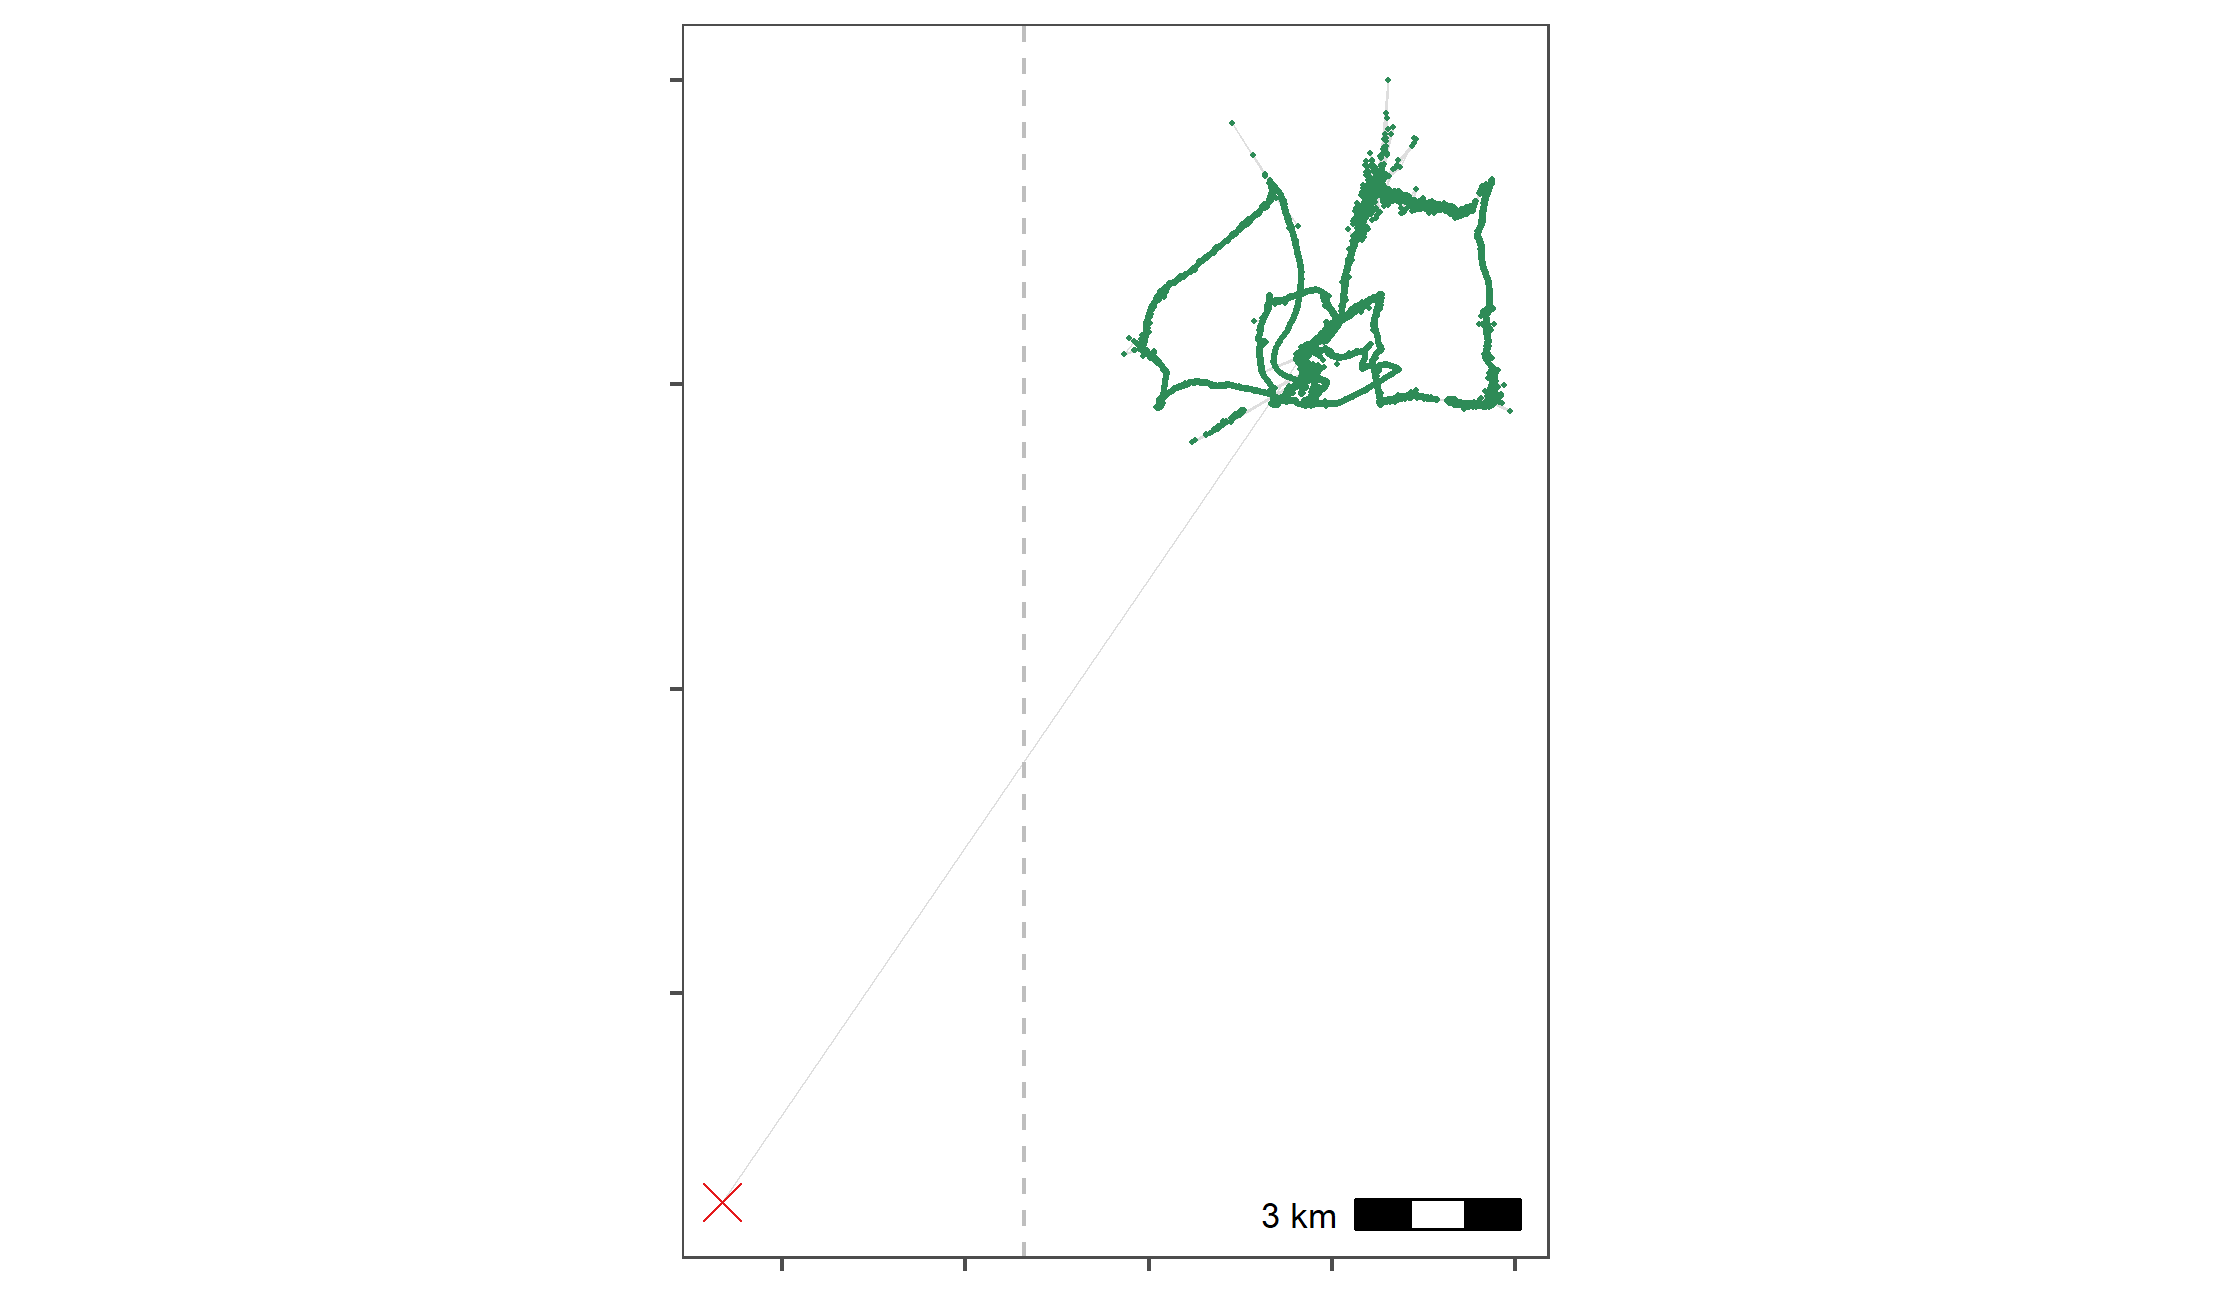
\includegraphics{figures/fig_calib_bbox.png}
\caption{Removal of a point outlier using the function \texttt{atl\_filter\_bounds}. The point outlier (black point) is removed based on its X coordinate value, with the data filtered to exclude positions with an X coordinate \textless{} 645,000 in the UTM 31N system. Positions that are retained are shown in green.}
\end{figure}

\hypertarget{filter-trajectories}{%
\subsection{Filter trajectories}\label{filter-trajectories}}

\hypertarget{handle-time}{%
\subsubsection{Handle time}\label{handle-time}}

Time in ATLAS tracking is counted in milliseconds and is represented by a 64-bit integer (type \texttt{long}), which is not natively supported in R; it will instead be converted to a \texttt{numeric}, or \texttt{double}.

This is not what is intended, but it works. The \texttt{bit64} package can help handle 64-bit integers if you want to keep to intended type.

A further issue is that 64-bit integers (whether represented as \texttt{bit64} or \texttt{double}) do not yield meaninful results when you try to convert them to a date-time object, such as of the class \texttt{POSIXct}.

This is because \texttt{as.POSIXct} fails when trying to work with 64-bit integers (it cannot interpret this type), and returns a date many thousands of years in the future (approx. 52,000 CE) if the time column is converted to \texttt{numeric}.

There are two possible solutions. The parsimonious one is to convert the 64-bit number to a 32-bit short integer (dividing by 1000), or to use the \texttt{nanotime} package.

The conversion method loses an imperceptible amount of precision. The \texttt{nanotime} requires installing another package. The first method is shown here.

In the spirit of not destroying data, we create a second lower-case column called \texttt{time}.

\begin{Shaded}
\begin{Highlighting}[]
\CommentTok{\# divide by 1000, convert to integer, then convert to POSIXct}
\NormalTok{data[, time }\OperatorTok{:}\ErrorTok{=}\StringTok{ }\KeywordTok{as.integer}\NormalTok{(TIME }\OperatorTok{/}\StringTok{ }\DecValTok{1000}\NormalTok{)]}
\end{Highlighting}
\end{Shaded}

\hypertarget{add-speed-and-turning-angle}{%
\subsubsection{Add speed and turning angle}\label{add-speed-and-turning-angle}}

\begin{Shaded}
\begin{Highlighting}[]
\CommentTok{\# add incoming and outgoing speed}
\NormalTok{data[, }\StringTok{\textasciigrave{}}\DataTypeTok{:=}\StringTok{\textasciigrave{}}\NormalTok{ (}\DataTypeTok{speed\_in =} \KeywordTok{atl\_get\_speed}\NormalTok{(data, }
                                      \DataTypeTok{x =} \StringTok{"x"}\NormalTok{, }
                                      \DataTypeTok{y =} \StringTok{"y"}\NormalTok{, }
                                      \DataTypeTok{time =} \StringTok{"time"}\NormalTok{),}
             \DataTypeTok{speed\_out =} \KeywordTok{atl\_get\_speed}\NormalTok{(data, }\DataTypeTok{type =} \StringTok{"out"}\NormalTok{))]}

\CommentTok{\# add turning angle}
\NormalTok{data[, angle }\OperatorTok{:}\ErrorTok{=}\StringTok{ }\KeywordTok{atl\_turning\_angle}\NormalTok{(}\DataTypeTok{data =}\NormalTok{ data)]}
\end{Highlighting}
\end{Shaded}

\hypertarget{get-95th-percentile-of-speed-and-angle}{%
\subsubsection{Get 95th percentile of speed and angle}\label{get-95th-percentile-of-speed-and-angle}}

\begin{Shaded}
\begin{Highlighting}[]
\CommentTok{\# use sapply}
\NormalTok{speed\_angle\_thresholds <{-}}\StringTok{ }
\StringTok{  }\KeywordTok{sapply}\NormalTok{(data[, }\KeywordTok{list}\NormalTok{(speed\_in, speed\_out, angle)], }
\NormalTok{       quantile, }\DataTypeTok{probs =} \FloatTok{0.9}\NormalTok{, }\DataTypeTok{na.rm =}\NormalTok{ T)}
\end{Highlighting}
\end{Shaded}

\hypertarget{filter-on-speed}{%
\subsubsection{Filter on speed}\label{filter-on-speed}}

Here we use a speed threshold of 15 m/s, the fastest known boat speed.
We then plot the data with the extreme speeds shown in grey, and the positions retained shown in green.

\begin{Shaded}
\begin{Highlighting}[]
\CommentTok{\# make a copy}
\NormalTok{data\_unproc <{-}}\StringTok{ }\KeywordTok{copy}\NormalTok{(data)}

\CommentTok{\# remove speed outliers}
\NormalTok{data <{-}}\StringTok{ }\KeywordTok{atl\_filter\_covariates}\NormalTok{(}\DataTypeTok{data =}\NormalTok{ data,}
            \DataTypeTok{filters =} \KeywordTok{c}\NormalTok{(}\StringTok{"(speed\_in < 15 \& speed\_out < 15)"}\NormalTok{))}

\CommentTok{\# recalculate speed and angle}
\NormalTok{data[, }\StringTok{\textasciigrave{}}\DataTypeTok{:=}\StringTok{\textasciigrave{}}\NormalTok{ (}\DataTypeTok{speed\_in =} \KeywordTok{atl\_get\_speed}\NormalTok{(data, }
                                      \DataTypeTok{x =} \StringTok{"x"}\NormalTok{, }
                                      \DataTypeTok{y =} \StringTok{"y"}\NormalTok{, }
                                      \DataTypeTok{time =} \StringTok{"time"}\NormalTok{),}
             \DataTypeTok{speed\_out =} \KeywordTok{atl\_get\_speed}\NormalTok{(data, }\DataTypeTok{type =} \StringTok{"out"}\NormalTok{))]}

\CommentTok{\# add turning angle}
\NormalTok{data[, angle }\OperatorTok{:}\ErrorTok{=}\StringTok{ }\KeywordTok{atl\_turning\_angle}\NormalTok{(}\DataTypeTok{data =}\NormalTok{ data)]}
\end{Highlighting}
\end{Shaded}

\begin{figure}
\centering
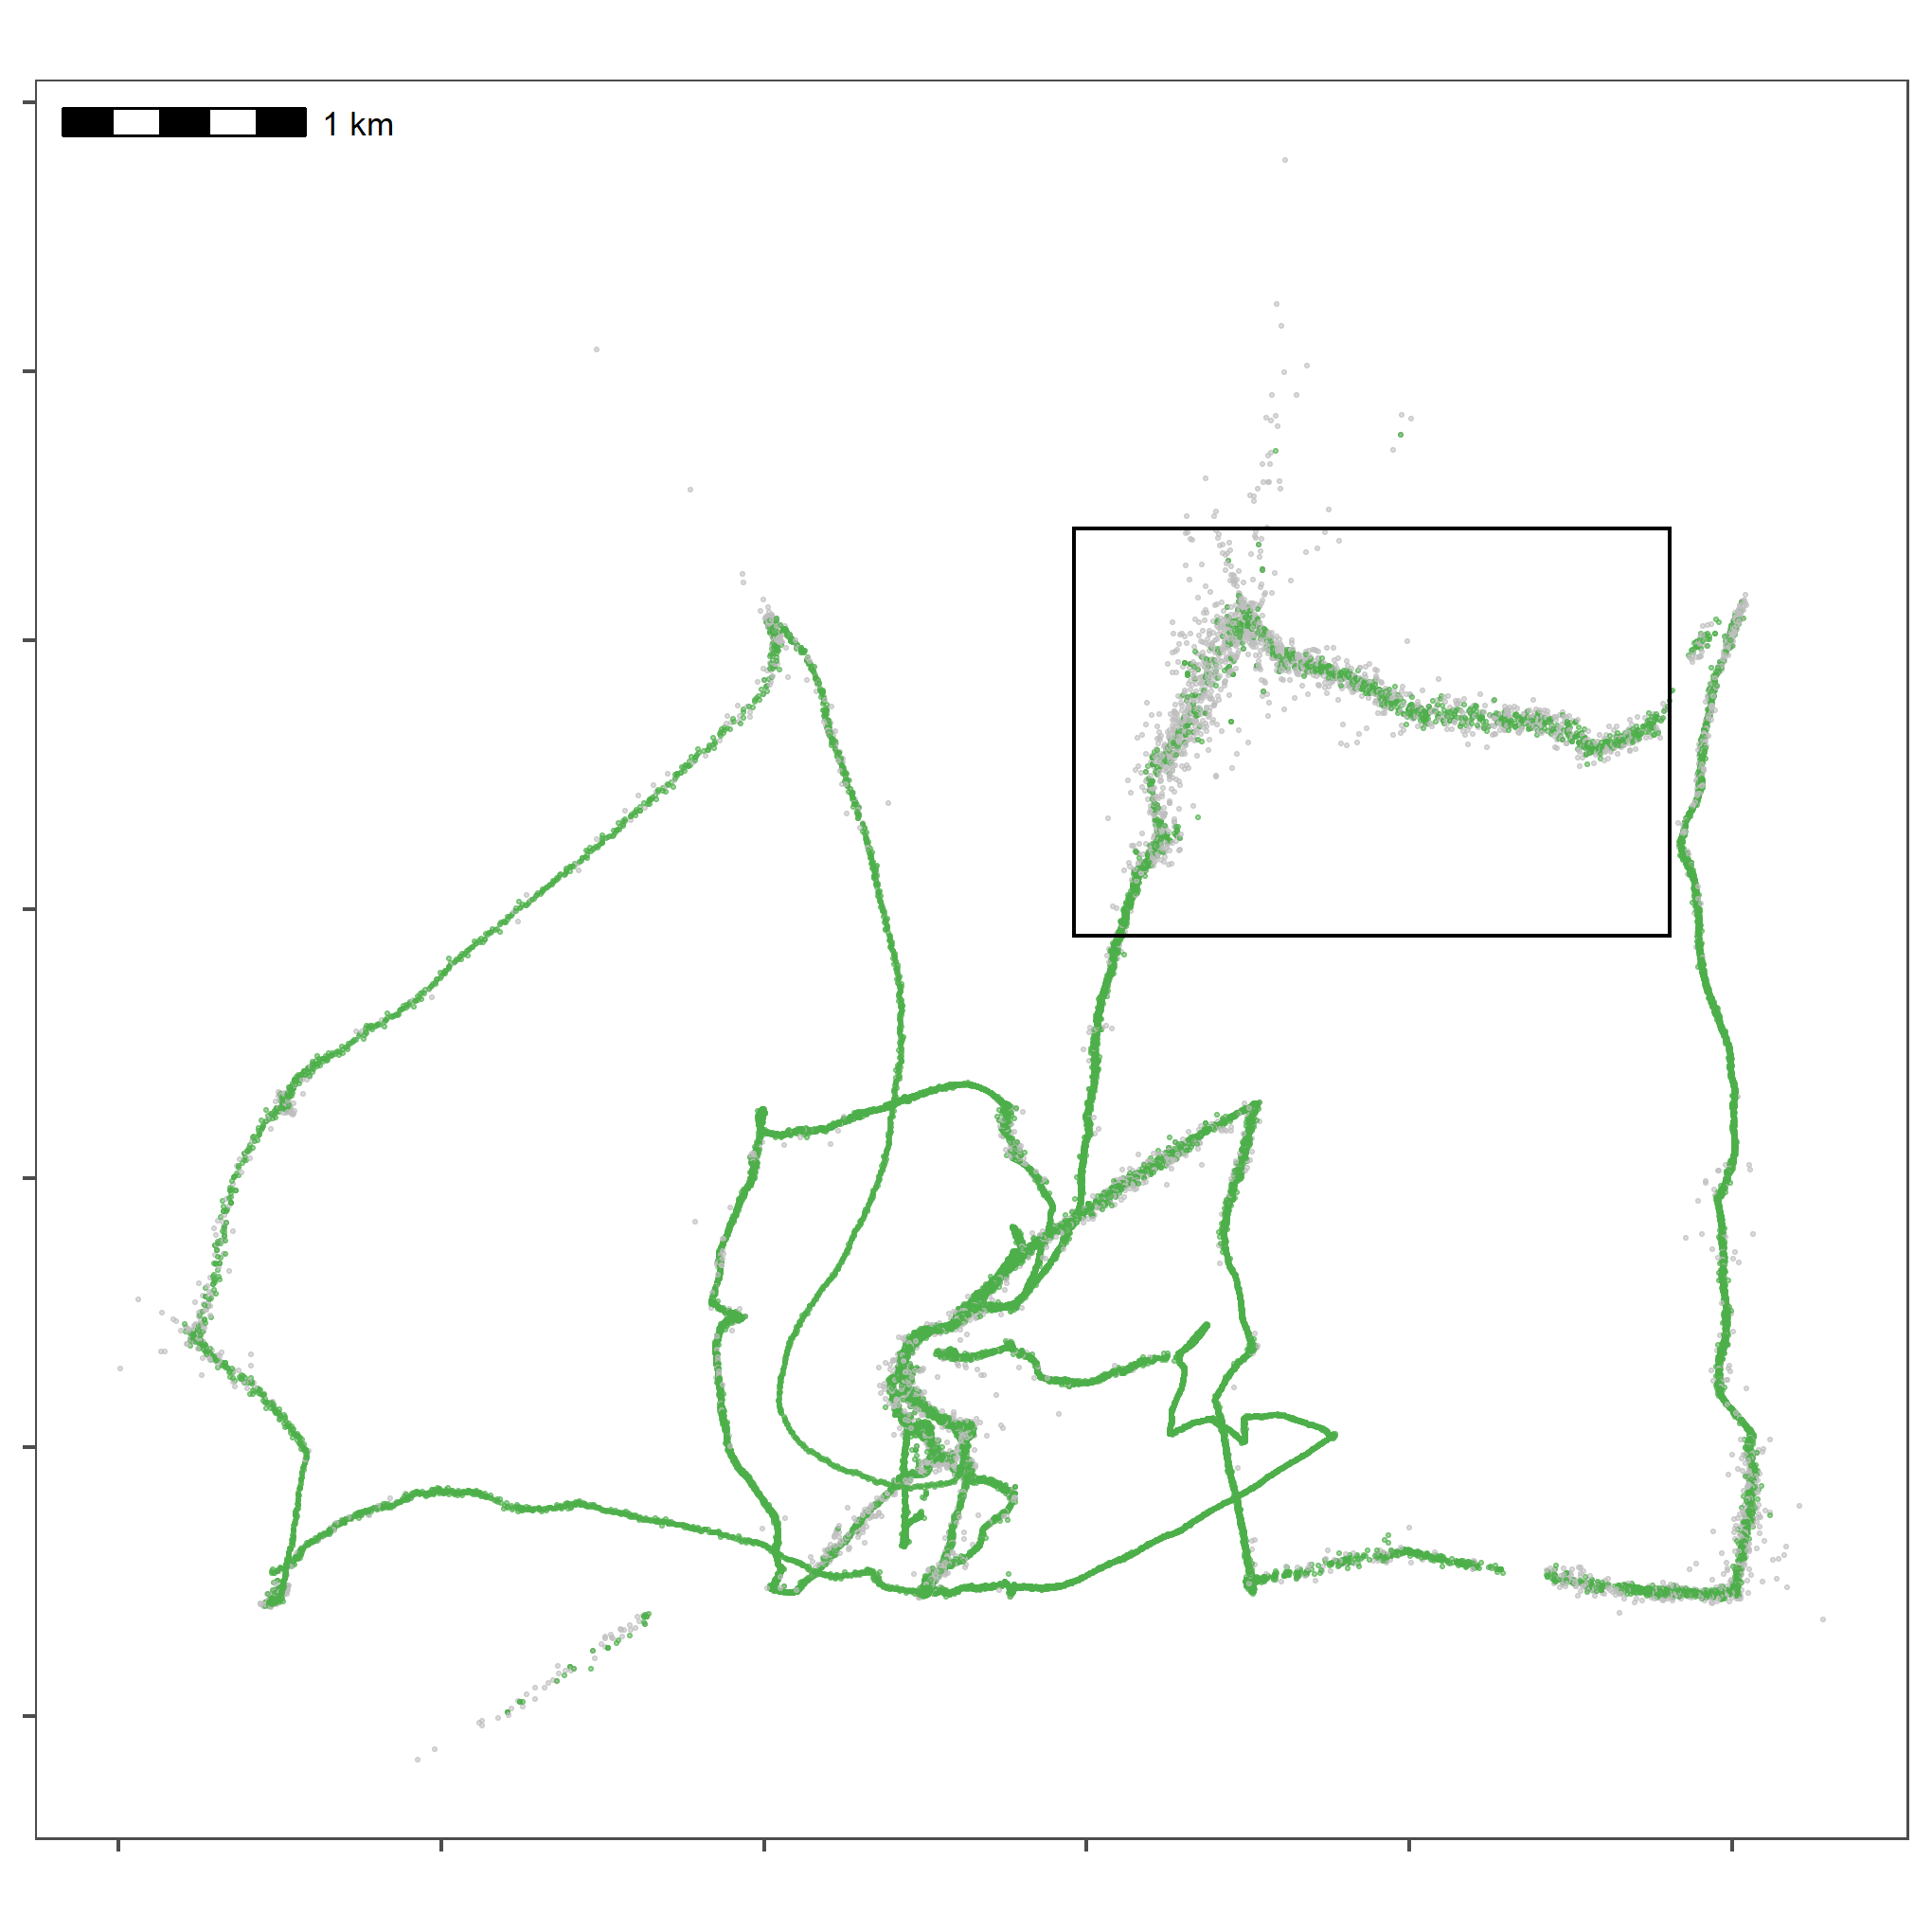
\includegraphics{figures/fig_speed_outlier.png}
\caption{Improving data quality by filtering out positions that would require unrealistic movement. We removed positions with speeds \(\geq\) 15 m/s, which is the fastest possible speed in this calibration data, part of which was collected in a moving boat around Griend. Grey positions are removed, while green positions are retained. Rectangles indicate areas expanded for visualisation in following figures.}
\end{figure}

\hypertarget{smoothing-the-trajectory}{%
\subsection{Smoothing the trajectory}\label{smoothing-the-trajectory}}

We then apply a median smooth over a moving window (\(K\) = 5).
This function modifies in place, and does not need to be assigned to a new variable.
We create a copy of the data before applying the smooth so that we can compare the data before and after smoothin.

\begin{Shaded}
\begin{Highlighting}[]
\CommentTok{\# apply a 5 point median smooth, first make a copy}
\NormalTok{data\_unproc <{-}}\StringTok{ }\KeywordTok{copy}\NormalTok{(data)}

\CommentTok{\# now apply the smooth}
\KeywordTok{atl\_median\_smooth}\NormalTok{(}\DataTypeTok{data =}\NormalTok{ data,}
                  \DataTypeTok{x =} \StringTok{"x"}\NormalTok{, }\DataTypeTok{y =} \StringTok{"y"}\NormalTok{, }\DataTypeTok{time =} \StringTok{"time"}\NormalTok{,}
                  \DataTypeTok{moving\_window =} \DecValTok{5}\NormalTok{)}
\end{Highlighting}
\end{Shaded}

\begin{figure}
\centering
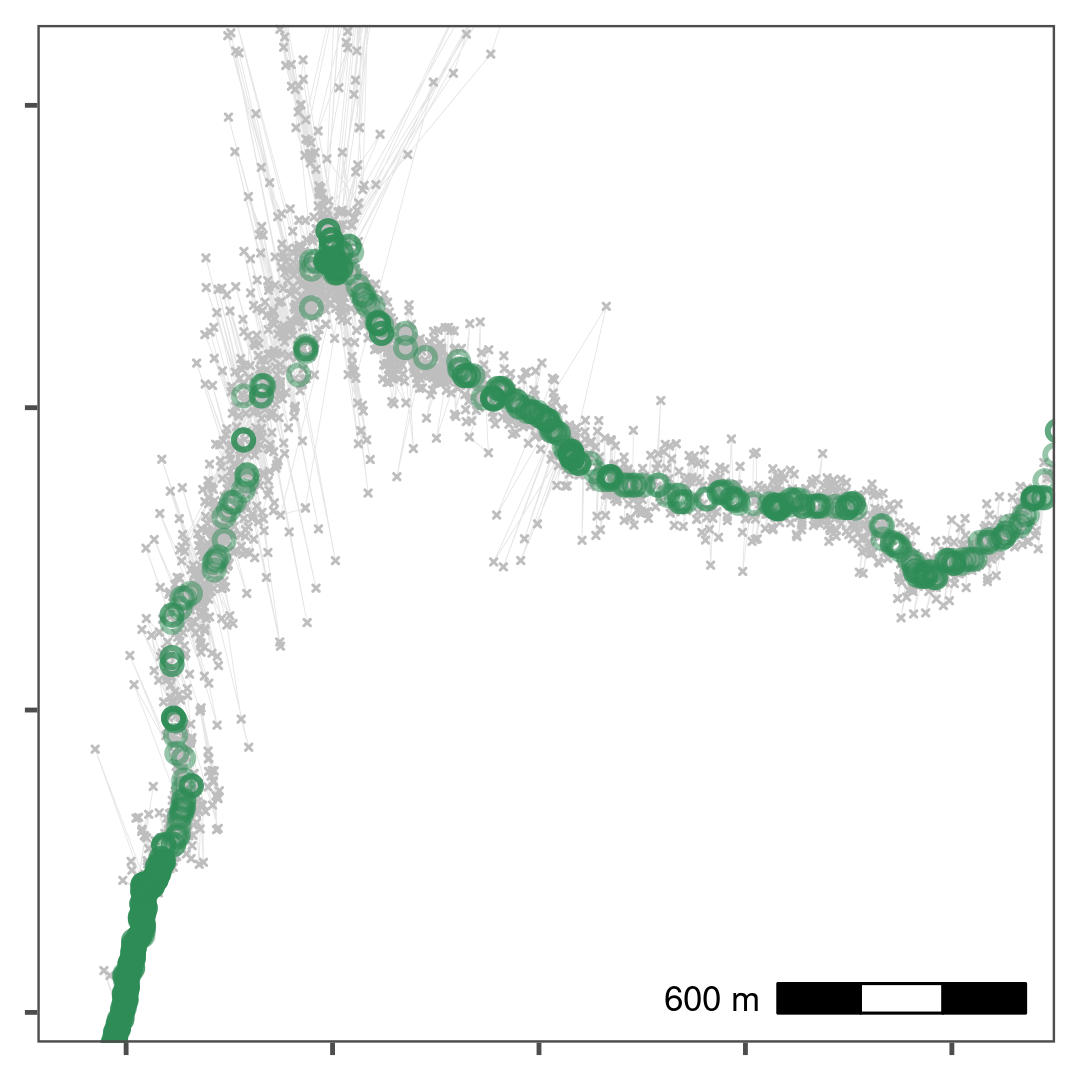
\includegraphics{figures/fig_calib_median_smooth.png}
\caption{Reducing small-scale location error using a median smooth with a moving window \(K\) = 5. Median smoothed positions are shown in green, while raw, unfiltered data is shown in grey. Median smoothing successfully recovers the likely path of the track without a loss of data. The area shown is the upper rectangle from Figure 3.}
\end{figure}

\hypertarget{thinning-the-data}{%
\subsection{Thinning the data}\label{thinning-the-data}}

Next we thin the data to demonstrate thinning by median smoothing.
Following this, we plot the median smooth and thinning by aggregation.

\begin{Shaded}
\begin{Highlighting}[]
\CommentTok{\# save a copy}
\NormalTok{data\_unproc <{-}}\StringTok{ }\KeywordTok{copy}\NormalTok{(data)}

\CommentTok{\# remove columns we don\textquotesingle{}t need}
\NormalTok{data <{-}}\StringTok{ }\NormalTok{data[, }\KeywordTok{setdiff}\NormalTok{(}\KeywordTok{colnames}\NormalTok{(data), }
                       \KeywordTok{c}\NormalTok{(}\StringTok{"tID"}\NormalTok{, }\StringTok{"Timestamp"}\NormalTok{, }\StringTok{"id"}\NormalTok{, }\StringTok{"TIME"}\NormalTok{, }\StringTok{"UTCtime"}\NormalTok{)), }
\NormalTok{             with =}\StringTok{ }\OtherTok{FALSE}\NormalTok{]}

\CommentTok{\# thin to a 30s interval}
\NormalTok{data\_thin <{-}}\StringTok{ }\KeywordTok{atl\_thin\_data}\NormalTok{(}\DataTypeTok{data =}\NormalTok{ data,}
                           \DataTypeTok{interval =} \DecValTok{30}\NormalTok{,}
                           \DataTypeTok{method =} \StringTok{"aggregate"}\NormalTok{,}
                           \DataTypeTok{id\_columns =} \StringTok{"TAG"}\NormalTok{)}
\end{Highlighting}
\end{Shaded}

\begin{figure}
\centering
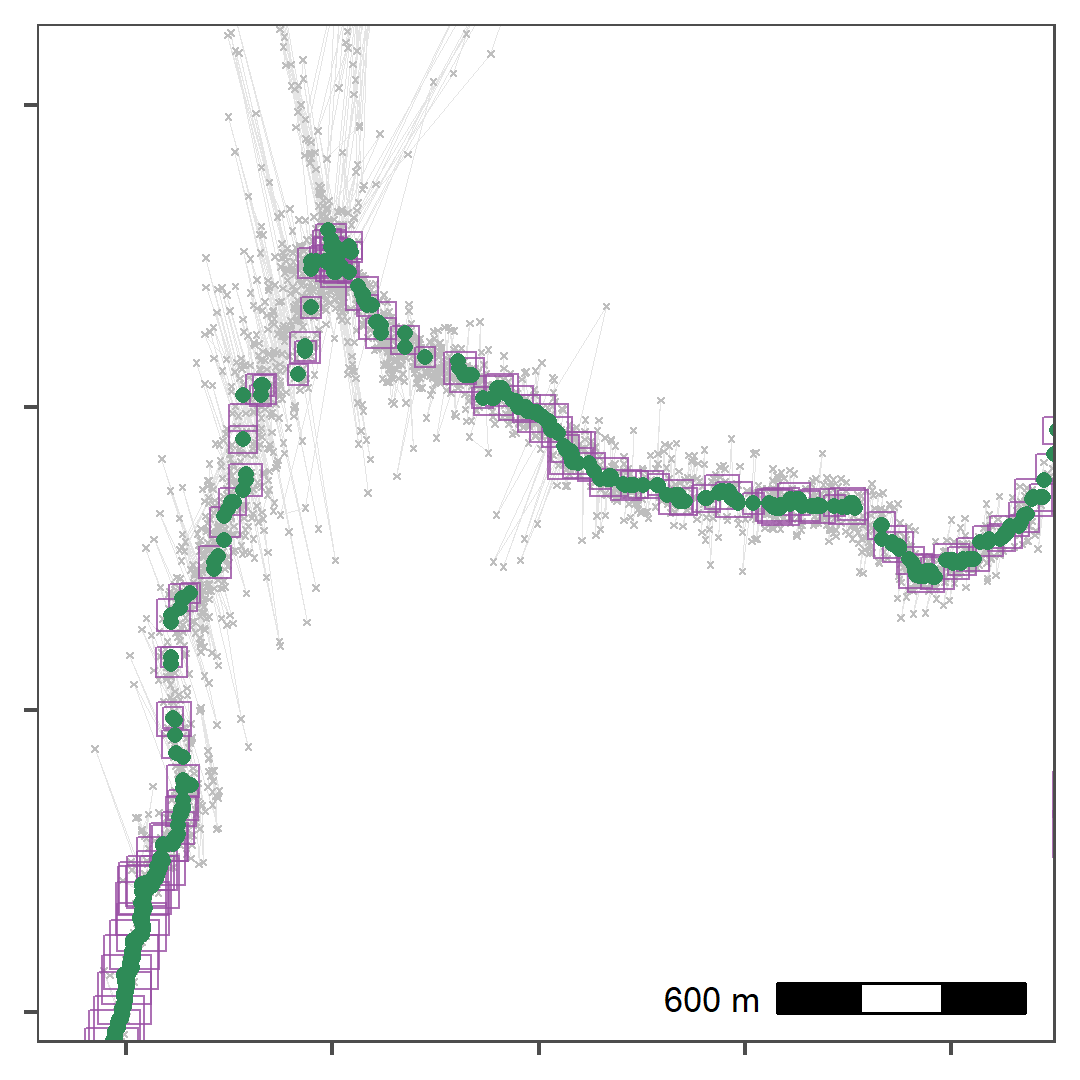
\includegraphics{figures/fig_calib_smooth_thin.png}
\caption{Thinning by aggregation over a 30 second interval (down from 1 second) preserves track structure while reducing the data volume for computation. Here, thinned positions are shown as purple squares, with the size of the square indicating the number of positions within the 30 second bin used to obtain the average position. Green points show the median smoothed data from Figure 4, while the raw data are shown in grey.}
\end{figure}

\hypertarget{residence-patches}{%
\subsection{Residence patches}\label{residence-patches}}

\hypertarget{get-waypoint-centroids}{%
\subsubsection{Get waypoint centroids}\label{get-waypoint-centroids}}

We subset the annotated calibration data to select the waypoints and the positions around them which are supposed to be the locations of known stops. Since each stop was supposed to be 5 minutes long, there are multiple points in each known stop.

\begin{Shaded}
\begin{Highlighting}[]
\KeywordTok{library}\NormalTok{(stringi)}
\NormalTok{data\_res <{-}}\StringTok{ }\NormalTok{data\_unproc[}\KeywordTok{stri\_detect}\NormalTok{(tID, }\DataTypeTok{regex =} \StringTok{"(WP)"}\NormalTok{)]}
\end{Highlighting}
\end{Shaded}

From this data, we get the centroid of known stops, and determine the time difference between the first and last point within 50 metres, and within 10 minutes of the waypoint positions' median time.

Essentially, this means that the maximum duration of a stop can be 20 minutes, and stops above this duration are not expected.

\begin{Shaded}
\begin{Highlighting}[]
\CommentTok{\# get centroid}
\NormalTok{data\_res\_summary <{-}}\StringTok{ }\NormalTok{data\_res[, }\KeywordTok{list}\NormalTok{(}\DataTypeTok{x\_median =} \KeywordTok{round}\NormalTok{(}\KeywordTok{median}\NormalTok{(x), }\DataTypeTok{digits =} \DecValTok{{-}2}\NormalTok{),}
                                    \DataTypeTok{y\_median =} \KeywordTok{round}\NormalTok{(}\KeywordTok{median}\NormalTok{(y), }\DataTypeTok{digits =} \DecValTok{{-}2}\NormalTok{)),}
\NormalTok{                                    t\_median =}\StringTok{ }\KeywordTok{median}\NormalTok{(time)}\ErrorTok{)}\NormalTok{,}
\NormalTok{                             by =}\StringTok{ "tID"}\NormalTok{]}

\CommentTok{\# now get times 10 mins before and after}
\NormalTok{data\_res\_summary[, }\StringTok{\textasciigrave{}}\DataTypeTok{:=}\StringTok{\textasciigrave{}}\NormalTok{(}\DataTypeTok{t\_min =}\NormalTok{ t\_median }\OperatorTok{{-}}\StringTok{ }\NormalTok{(}\DecValTok{10} \OperatorTok{*}\StringTok{ }\DecValTok{60}\NormalTok{),}
                        \DataTypeTok{t\_max =}\NormalTok{ t\_median }\OperatorTok{+}\StringTok{ }\NormalTok{(}\DecValTok{10} \OperatorTok{*}\StringTok{ }\DecValTok{60}\NormalTok{))]}

\CommentTok{\# make a list of positions 10min before and after}
\NormalTok{wp\_data <{-}}\StringTok{ }\KeywordTok{mapply}\NormalTok{(}\ControlFlowTok{function}\NormalTok{(l, u, mx, my) \{}
\NormalTok{  tmp\_data <{-}}\StringTok{ }\NormalTok{data\_unproc[}\KeywordTok{inrange}\NormalTok{(time, l, u)]}
\NormalTok{  tmp\_data[, distance }\OperatorTok{:}\ErrorTok{=}\StringTok{ }\KeywordTok{sqrt}\NormalTok{((mx }\OperatorTok{{-}}\StringTok{ }\NormalTok{x)}\OperatorTok{\^{}}\DecValTok{2} \OperatorTok{+}\StringTok{ }\NormalTok{(my }\OperatorTok{{-}}\StringTok{ }\NormalTok{y)}\OperatorTok{\^{}}\DecValTok{2}\NormalTok{)]}
  
  \CommentTok{\# keep within 50}
\NormalTok{  tmp\_data <{-}}\StringTok{ }\NormalTok{tmp\_data[distance }\OperatorTok{<=}\StringTok{ }\DecValTok{50}\NormalTok{, ]}
  
  \CommentTok{\# get duration}
  \KeywordTok{return}\NormalTok{(}\KeywordTok{diff}\NormalTok{(}\KeywordTok{range}\NormalTok{(tmp\_data}\OperatorTok{$}\NormalTok{time)))}
  
\NormalTok{\}, data\_res\_summary}\OperatorTok{$}\NormalTok{t\_min, data\_res\_summary}\OperatorTok{$}\NormalTok{t\_max,}
\NormalTok{   data\_res\_summary}\OperatorTok{$}\NormalTok{x\_median, data\_res\_summary}\OperatorTok{$}\NormalTok{y\_median,}
\DataTypeTok{SIMPLIFY =} \OtherTok{TRUE}\NormalTok{)}
\end{Highlighting}
\end{Shaded}

\hypertarget{prepare-data}{%
\subsubsection{Prepare data}\label{prepare-data}}

An indicator of individual residence at or near a position can be useful when attempting to identify residence patches. Positions can be filtered on a metric such as residence time (Bracis, Bildstein, and Mueller \protect\hyperlink{ref-bracis2018}{2018}).

\hypertarget{calculate-residence-time}{%
\subsubsection{Calculate residence time}\label{calculate-residence-time}}

First we calculate the residence time with a radius of 50 metres.
For this, we need a dataframe with coordinates, the timestamp, and the animal id.
We save this data to file for later use.

\begin{Shaded}
\begin{Highlighting}[]
\CommentTok{\# load recurse}
\KeywordTok{library}\NormalTok{(recurse)}
\end{Highlighting}
\end{Shaded}

\begin{Shaded}
\begin{Highlighting}[]
\CommentTok{\# get 4 column data}
\NormalTok{data\_for\_patch <{-}}\StringTok{ }\NormalTok{data\_thin[, }\KeywordTok{list}\NormalTok{(x, y, time, TAG)]}

\CommentTok{\# get recurse data for a 10m radius}
\NormalTok{recurse\_stats <{-}}\StringTok{ }\KeywordTok{getRecursions}\NormalTok{(data\_for\_patch,}
                               \DataTypeTok{radius =} \DecValTok{50}\NormalTok{, }\DataTypeTok{timeunits =} \StringTok{"mins"}\NormalTok{)}

\CommentTok{\# assign to recurse data}
\NormalTok{data\_for\_patch[, res\_time }\OperatorTok{:}\ErrorTok{=}\StringTok{ }\NormalTok{recurse\_stats}\OperatorTok{$}\NormalTok{residenceTime]}

\CommentTok{\# save recurse data}
\KeywordTok{fwrite}\NormalTok{(data\_for\_patch, }\DataTypeTok{file =} \StringTok{"data/data\_calib\_for\_patch.csv"}\NormalTok{)}
\end{Highlighting}
\end{Shaded}

\hypertarget{run-residence-patch-method}{%
\subsubsection{Run residence patch method}\label{run-residence-patch-method}}

We subset data with a residence time \textgreater{} 5 minutes in order to construct residence patches.
From this subset, we construct residence patches using the parameters: \texttt{buffer\_radius} = 5 metres, \texttt{lim\_spat\_indep} = 50 metres, \texttt{lim\_time\_indep} = 5 minutes, and \texttt{min\_fixes} = 3.

\begin{Shaded}
\begin{Highlighting}[]
\CommentTok{\# assign id as tag}
\NormalTok{data\_for\_patch[, id }\OperatorTok{:}\ErrorTok{=}\StringTok{ }\KeywordTok{as.character}\NormalTok{(TAG)]}

\CommentTok{\# on known residence points}
\NormalTok{patch\_res\_known <{-}}\StringTok{ }\KeywordTok{atl\_res\_patch}\NormalTok{(data\_for\_patch[res\_time }\OperatorTok{>=}\StringTok{ }\DecValTok{5}\NormalTok{, ], }
                                \DataTypeTok{buffer\_radius =} \DecValTok{5}\NormalTok{,}
                                \DataTypeTok{lim\_spat\_indep =} \DecValTok{50}\NormalTok{,}
                                \DataTypeTok{lim\_time\_indep =} \DecValTok{5}\NormalTok{,}
                                \DataTypeTok{min\_fixes =} \DecValTok{3}\NormalTok{)}
\end{Highlighting}
\end{Shaded}

\hypertarget{get-spatial-and-summary-objects}{%
\subsubsection{Get spatial and summary objects}\label{get-spatial-and-summary-objects}}

We get spatial and summary ouput of the residence patch method using the \texttt{atl\_patch\_summary} function using the options \texttt{which\_data} = ``spatial'' and \texttt{which\_data} = "summary.
We use a buffer radius here of 20 metres for the spatial buffer, despite using a buffer radius of 5 metres earlier, simply because it is easier to visualise in the output figure.

\begin{Shaded}
\begin{Highlighting}[]
\CommentTok{\# for the known and unkniwn patches}
\NormalTok{patch\_sf\_data <{-}}\StringTok{ }\KeywordTok{atl\_patch\_summary}\NormalTok{(patch\_res\_known, }
                                   \DataTypeTok{which\_data =} \StringTok{"spatial"}\NormalTok{,}
                                   \DataTypeTok{buffer\_radius =} \DecValTok{20}\NormalTok{)}

\CommentTok{\# assign crs}
\NormalTok{sf}\OperatorTok{::}\KeywordTok{st\_crs}\NormalTok{(patch\_sf\_data) <{-}}\StringTok{ }\DecValTok{32631}

\CommentTok{\# get summary data}
\NormalTok{patch\_summary\_data <{-}}\StringTok{ }\KeywordTok{atl\_patch\_summary}\NormalTok{(patch\_res\_known, }
                                        \DataTypeTok{which\_data =} \StringTok{"summary"}\NormalTok{)}
\end{Highlighting}
\end{Shaded}

\hypertarget{prepare-to-plot-data}{%
\subsubsection{Prepare to plot data}\label{prepare-to-plot-data}}

We read in the island's shapefile to plot it as a background for the residence patch figure.

\begin{Shaded}
\begin{Highlighting}[]
\CommentTok{\# read griend}
\NormalTok{griend <{-}}\StringTok{ }\NormalTok{sf}\OperatorTok{::}\KeywordTok{st\_read}\NormalTok{(}\StringTok{"data/griend\_polygon/griend\_polygon.shp"}\NormalTok{)}
\end{Highlighting}
\end{Shaded}

\begin{figure}
\centering
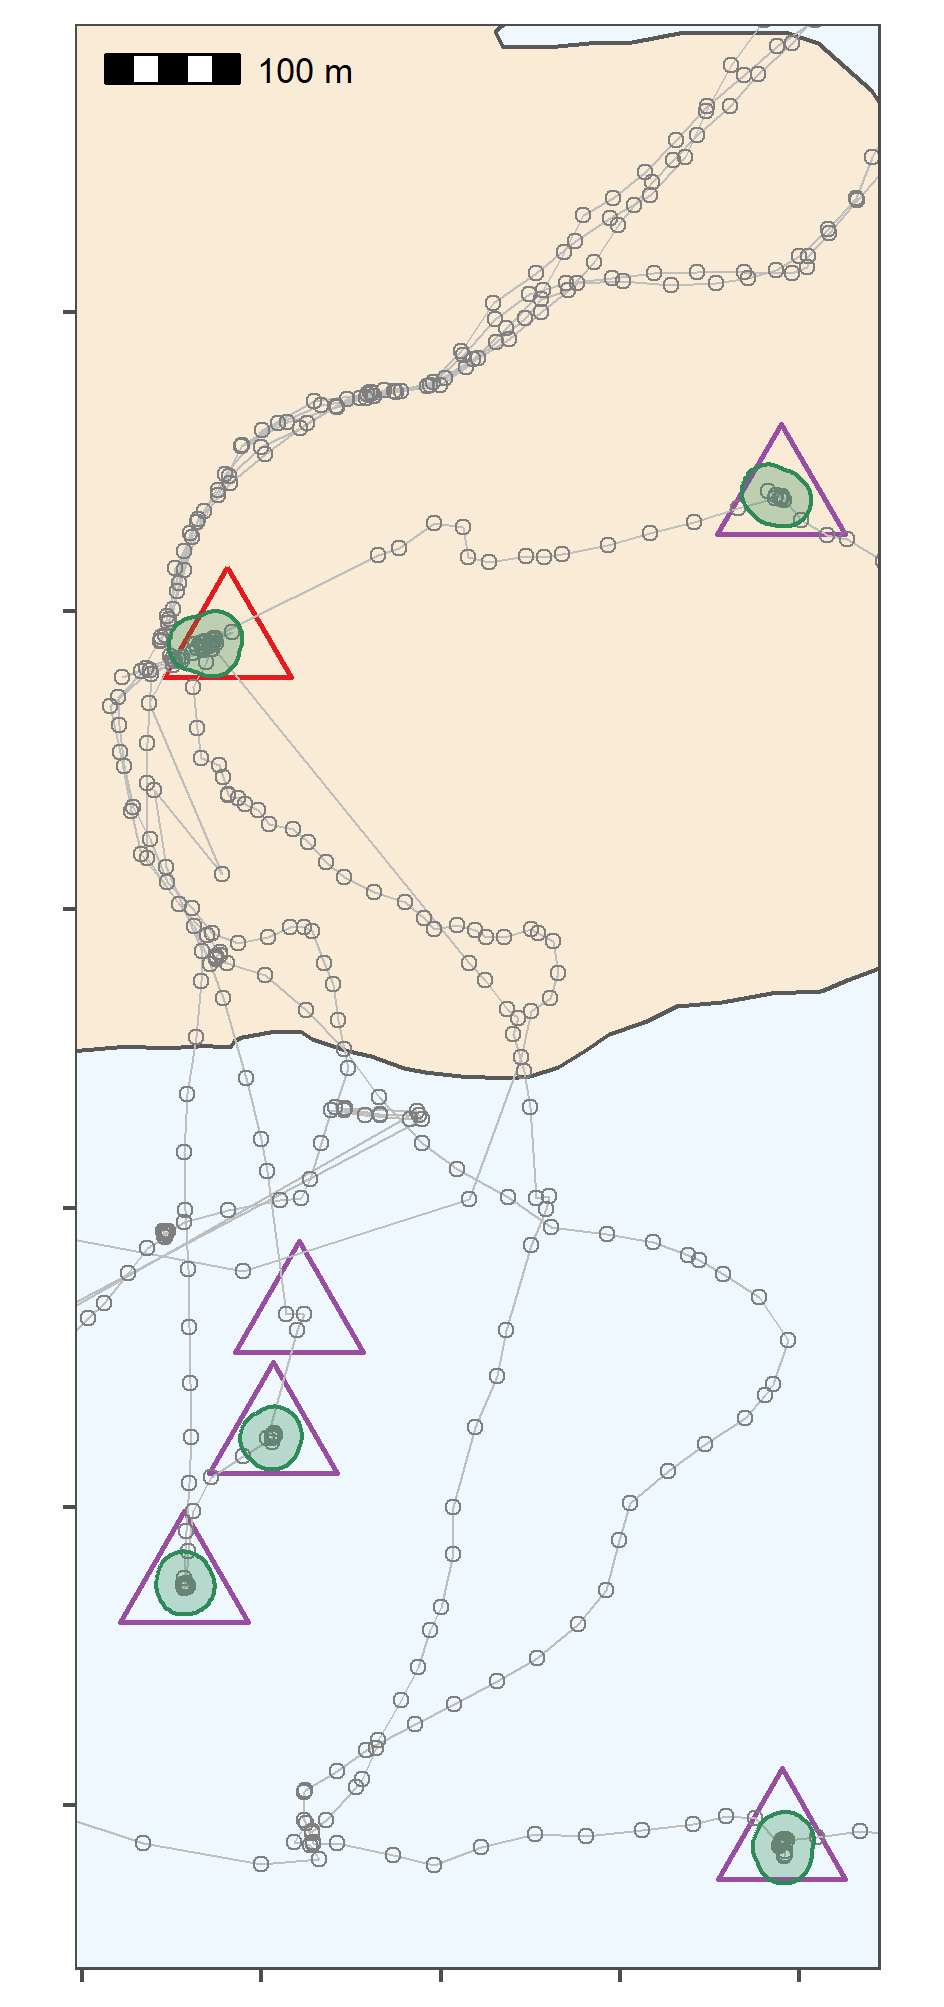
\includegraphics{figures/fig_calib_residence.png}
\caption{Classifying thinned data into residence patches yields robust estimates of the duration of known stops. The island of Griend (53.25\(^{\circ}\)N, 5.25\(^{\circ}\)E) is shown in beige. Residence patches (green polygons; function parameters in text) correspond well to the locations of known stops (purple crossed-squares). However, the algorithm identified all areas with prolonged residence, including those which were not intended stops (n = 12; green polygons without crossed-squares). The algorithm also failed to find two stops of 6 and 15 seconds duration, since these were lost in the data thinning step (crossed-square without green polygon shows one of these).}
\end{figure}

\hypertarget{compare-patch-metrics}{%
\subsection{Compare patch metrics}\label{compare-patch-metrics}}

We then merge the annoated, known stop data with the calculated patch duration.
We filter this data to exclude one exceedingly long outlier of about an hour (WP080), which how

\begin{Shaded}
\begin{Highlighting}[]
\CommentTok{\# get known patch summary}
\NormalTok{data\_res <{-}}\StringTok{ }\NormalTok{data\_unproc[stringi}\OperatorTok{::}\KeywordTok{stri\_detect}\NormalTok{(tID, }\DataTypeTok{regex =} \StringTok{"(WP)"}\NormalTok{), ]}

\CommentTok{\# get waypoint summary}
\NormalTok{patch\_summary\_real <{-}}\StringTok{ }\NormalTok{data\_res[, }\KeywordTok{list}\NormalTok{(}\DataTypeTok{nfixes\_real =}\NormalTok{ .N,}
                                      \DataTypeTok{x\_median =} \KeywordTok{round}\NormalTok{(}\KeywordTok{median}\NormalTok{(x), }\DataTypeTok{digits =} \DecValTok{{-}2}\NormalTok{),}
                                      \DataTypeTok{y\_median =} \KeywordTok{round}\NormalTok{(}\KeywordTok{median}\NormalTok{(y), }\DataTypeTok{digits =} \DecValTok{{-}2}\NormalTok{)), }
\NormalTok{                               by =}\StringTok{ "tID"}\NormalTok{]}

\CommentTok{\# add real duration}
\NormalTok{patch\_summary\_real[, duration\_real }\OperatorTok{:}\ErrorTok{=}\StringTok{ }\NormalTok{wp\_data]}

\CommentTok{\# round median coordinate for inferred patches}
\NormalTok{patch\_summary\_inferred <{-}}\StringTok{ }
\StringTok{  }\NormalTok{patch\_summary\_data[, }
                     \KeywordTok{c}\NormalTok{(}\StringTok{"x\_median"}\NormalTok{, }\StringTok{"y\_median"}\NormalTok{, }
                       \StringTok{"nfixes"}\NormalTok{, }\StringTok{"duration"}\NormalTok{, }\StringTok{"patch"}\NormalTok{)}
\NormalTok{                     ][, }\StringTok{\textasciigrave{}}\DataTypeTok{:=}\StringTok{\textasciigrave{}}\NormalTok{(}\DataTypeTok{x\_median =} \KeywordTok{round}\NormalTok{(x\_median, }\DataTypeTok{digits =} \DecValTok{{-}2}\NormalTok{),}
                              \DataTypeTok{y\_median =} \KeywordTok{round}\NormalTok{(y\_median, }\DataTypeTok{digits =} \DecValTok{{-}2}\NormalTok{))]}

\CommentTok{\# join with respatch summary}
\NormalTok{patch\_summary\_compare <{-}}\StringTok{ }
\StringTok{  }\KeywordTok{merge}\NormalTok{(patch\_summary\_real,}
\NormalTok{        patch\_summary\_inferred, }
        \DataTypeTok{on =} \KeywordTok{c}\NormalTok{(}\StringTok{"x\_median"}\NormalTok{, }\StringTok{"y\_median"}\NormalTok{),}
        \DataTypeTok{all.x =} \OtherTok{TRUE}\NormalTok{, }\DataTypeTok{all.y =} \OtherTok{TRUE}\NormalTok{)}

\CommentTok{\# drop nas}
\NormalTok{patch\_summary\_compare <{-}}\StringTok{ }\KeywordTok{na.omit}\NormalTok{(patch\_summary\_compare)}

\CommentTok{\# drop patch around WP080}
\NormalTok{patch\_summary\_compare <{-}}\StringTok{ }\NormalTok{patch\_summary\_compare[tID }\OperatorTok{!=}\StringTok{ "WP080"}\NormalTok{, ]}
\end{Highlighting}
\end{Shaded}

7 patches are identified where there are no waypoints, while 2 waypoints are not identified as patches. These waypoints consisted of 6 and 15 (WP098 and WP092) positions respectively, and were lost when the data were aggregated to 30 second intervals.

\hypertarget{linear-model-durations}{%
\subsubsection{Linear model durations}\label{linear-model-durations}}

We run a simple linear model.

\begin{Shaded}
\begin{Highlighting}[]
\CommentTok{\# get linear model}
\NormalTok{model\_duration <{-}}\StringTok{ }\KeywordTok{lm}\NormalTok{(duration\_real }\OperatorTok{\textasciitilde{}}\StringTok{ }\NormalTok{duration,}
                     \DataTypeTok{data =}\NormalTok{ patch\_summary\_compare)}

\CommentTok{\# get R2}
\KeywordTok{summary}\NormalTok{(model\_duration)}

\CommentTok{\# write to file}
\KeywordTok{writeLines}\NormalTok{(}
  \DataTypeTok{text =} \KeywordTok{capture.output}\NormalTok{(}
    \KeywordTok{summary}\NormalTok{(model\_duration)}
\NormalTok{  ),}
  \DataTypeTok{con =} \StringTok{"data/model\_output\_residence\_patch.txt"}
\NormalTok{)}
\end{Highlighting}
\end{Shaded}

\begin{figure}
\centering
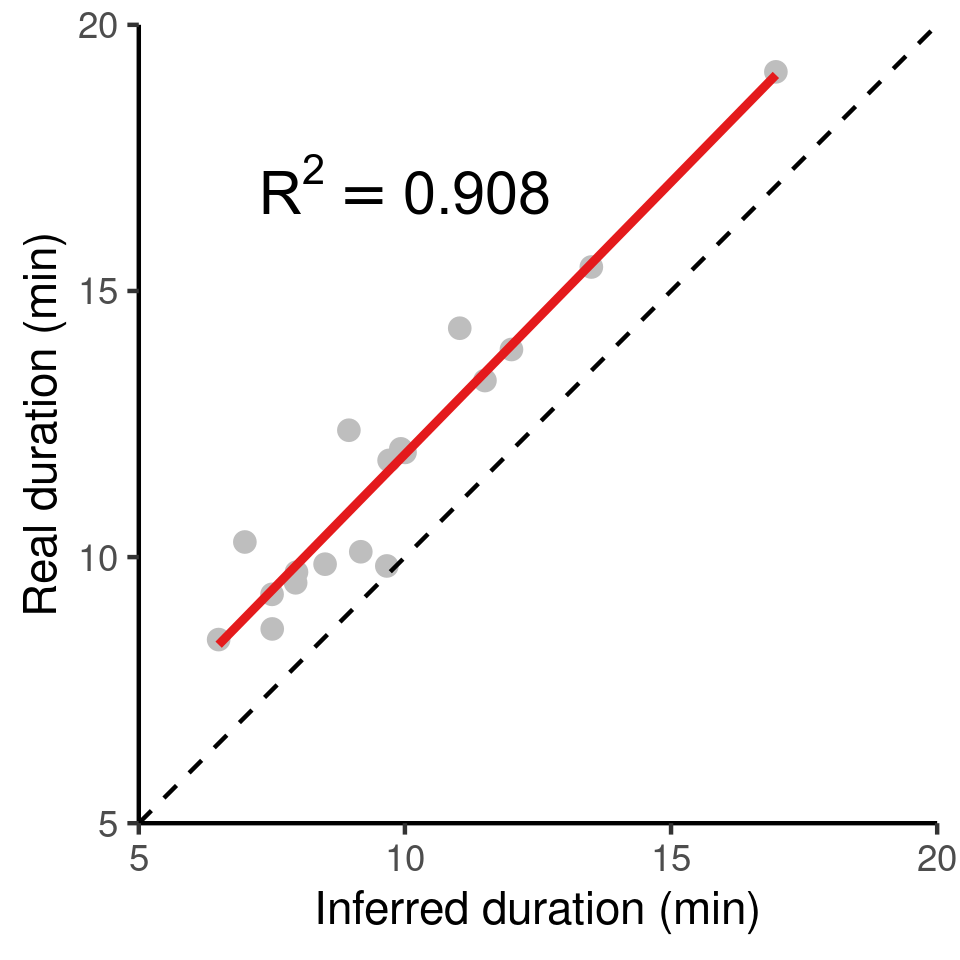
\includegraphics{figures/fig_calib_lm_duration.png}
\caption{The inferred duration of residence patches corresponds very closely to the real duration (grey circles, red line shows linear model fit), with an underestimation of the true duration of around 2\%. The dashed black line represents \(y = x\) for reference.}
\end{figure}

\hypertarget{linear-model-summary}{%
\subsubsection{Linear model summary}\label{linear-model-summary}}

\begin{Shaded}
\begin{Highlighting}[]
\KeywordTok{cat}\NormalTok{(}
  \KeywordTok{readLines}\NormalTok{(}
    \DataTypeTok{con =} \StringTok{"data/model\_output\_residence\_patch.txt"}
\NormalTok{  ), }\DataTypeTok{sep =} \StringTok{"}\CharTok{\textbackslash{}n}\StringTok{"}
\NormalTok{)}
\end{Highlighting}
\end{Shaded}

\hypertarget{processing-egyptian-fruit-bat-tracks}{%
\section{Processing Egyptian fruit bat tracks}\label{processing-egyptian-fruit-bat-tracks}}

We show the pre-processing pipeline at work on the tracks of three Egyptian fruit bats (\emph{Rousettus aegyptiacus}), and construct residence patches.

\hypertarget{prepare-libraries}{%
\subsection{Prepare libraries}\label{prepare-libraries}}

Install the required \texttt{R} libraries that are required from CRAN if not already installed.

\begin{Shaded}
\begin{Highlighting}[]
\CommentTok{\# load libs}
\KeywordTok{library}\NormalTok{(data.table)}
\KeywordTok{library}\NormalTok{(RSQLite)}
\KeywordTok{library}\NormalTok{(ggplot2)}
\KeywordTok{library}\NormalTok{(patchwork)}

\CommentTok{\# prepare a palette}
\NormalTok{pal <{-}}\StringTok{ }\NormalTok{RColorBrewer}\OperatorTok{::}\KeywordTok{brewer.pal}\NormalTok{(}\DecValTok{4}\NormalTok{, }\StringTok{"Set1"}\NormalTok{)}
\end{Highlighting}
\end{Shaded}

\hypertarget{install-atlastools-from-github.}{%
\subsection{\texorpdfstring{Install \texttt{atlastools} from Github.}{Install atlastools from Github.}}\label{install-atlastools-from-github.}}

\texttt{atlastools} is available from Github and is archived on Zenodo (Gupte \protect\hyperlink{ref-gupte2020a}{2020}).
It can be installed using \texttt{remotes} or \texttt{devtools}. Here we use the \texttt{remotes} function \texttt{install\_github}.

\begin{Shaded}
\begin{Highlighting}[]
\KeywordTok{install.packages}\NormalTok{(}\StringTok{"remotes"}\NormalTok{)}

\CommentTok{\# installation using remotes}
\NormalTok{remotes}\OperatorTok{::}\KeywordTok{install\_github}\NormalTok{(}\StringTok{"pratikunterwegs/atlastools"}\NormalTok{)}
\end{Highlighting}
\end{Shaded}

\hypertarget{read-bat-data}{%
\subsection{Read bat data}\label{read-bat-data}}

Read the bat data from an \texttt{SQLite} database local file and convert to a plain text csv file.
This data can be found in the ``data'' folder.

\begin{Shaded}
\begin{Highlighting}[]
\CommentTok{\# prepare the connection}
\NormalTok{con <{-}}\StringTok{ }\KeywordTok{dbConnect}\NormalTok{(}\DataTypeTok{drv =} \KeywordTok{SQLite}\NormalTok{(), }
                 \DataTypeTok{dbname =} \StringTok{"data/Three\_example\_bats.sql"}\NormalTok{)}

\CommentTok{\# list the tables}
\NormalTok{table\_name <{-}}\StringTok{ }\KeywordTok{dbListTables}\NormalTok{(con)}

\CommentTok{\# prepare to query all tables}
\NormalTok{query <{-}}\StringTok{ }\KeywordTok{sprintf}\NormalTok{(}\StringTok{\textquotesingle{}select * from }\CharTok{\textbackslash{}"}\StringTok{\%s}\CharTok{\textbackslash{}"}\StringTok{\textquotesingle{}}\NormalTok{, table\_name)}

\CommentTok{\# query the database}
\NormalTok{data <{-}}\StringTok{ }\KeywordTok{dbGetQuery}\NormalTok{(}\DataTypeTok{conn =}\NormalTok{ con, }\DataTypeTok{statement =}\NormalTok{ query)}

\CommentTok{\# disconnect from database}
\KeywordTok{dbDisconnect}\NormalTok{(con)}
\end{Highlighting}
\end{Shaded}

Convert data to csv, and save a local copy in the folder ``data''.

\begin{Shaded}
\begin{Highlighting}[]
\CommentTok{\# convert data to datatable}
\KeywordTok{setDT}\NormalTok{(data)}

\CommentTok{\# write data for QGIS}
\KeywordTok{fwrite}\NormalTok{(data, }\DataTypeTok{file =} \StringTok{"data/bat\_data.csv"}\NormalTok{)}
\end{Highlighting}
\end{Shaded}

\hypertarget{a-first-visual-inspection}{%
\subsection{A First Visual Inspection}\label{a-first-visual-inspection}}

Plot the bat data as a sanity check, and inspect it visually for errors (Figure 1).
The plot code is hidden in the rendered copy (PDF) of this supplementary material, but is available in the \texttt{Rmarkdown} file ``06\_bat\_data.Rmd''.
The saved plot is shown below as Figure 1.

\begin{figure}
\centering
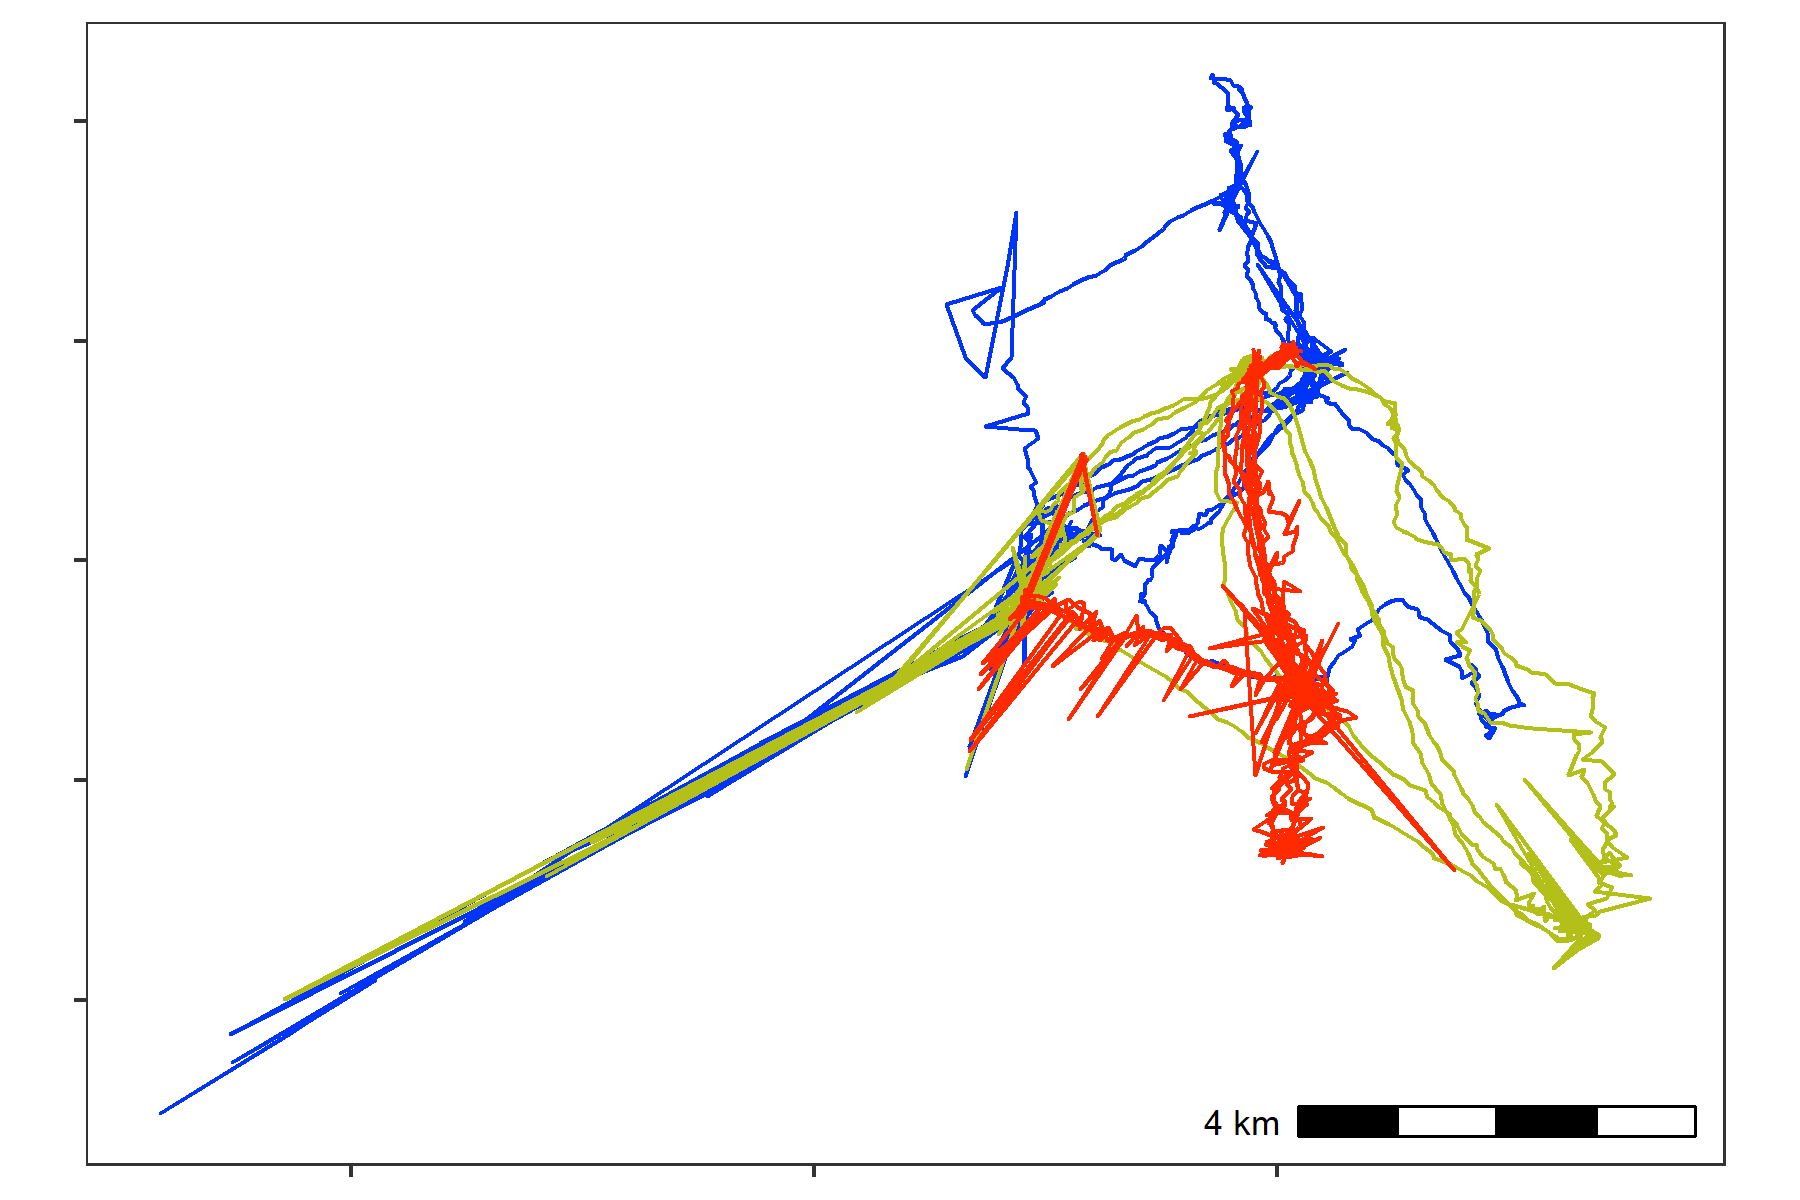
\includegraphics{figures/fig_bat_raw.png}
\caption{Movement data from three Egyptian fruit bats tracked using the ATLAS system (\emph{Rousettus aegyptiacus}; (Toledo et al. \protect\hyperlink{ref-toledo2020}{2020}; Shohami and Nathan \protect\hyperlink{ref-shohami2020}{2020})).
The bats were tracked in the Hula Valley, Israel (33.1\(^{\circ}\)N, 35.6\(^{\circ}\)E), and we use three nights of tracking (5\textsuperscript{th}, 6\textsuperscript{th}, and 7\textsuperscript{th} May, 2018), for our demonstration, with an average of 13,370 positions (SD = 2,173; range = 11,195 -- 15,542; interval = 8 seconds) per individual.
After first plotting the individual tracks, we notice severe distortions, making pre-processing necesary}
\end{figure}

\hypertarget{prepare-data-for-filtering}{%
\subsection{Prepare data for filtering}\label{prepare-data-for-filtering}}

Here we apply a series of simple filters.
It is always safer to deal with one individual at a time, so we split the data.table
into a list of data.tables to avoid mixups among individuals.

\hypertarget{prepare-data-per-individual}{%
\subsubsection{Prepare data per individual}\label{prepare-data-per-individual}}

\begin{Shaded}
\begin{Highlighting}[]
\CommentTok{\# split bat data by tag}
\CommentTok{\# first make a copy using the data.table function copy}
\CommentTok{\# this prevents the orignal data from being modified by atlastools}
\CommentTok{\# functions which DO MODIFY BY REFERENCE!}
\NormalTok{data\_split <{-}}\StringTok{ }\KeywordTok{copy}\NormalTok{(data)}

\CommentTok{\# now split}
\NormalTok{data\_split <{-}}\StringTok{ }\KeywordTok{split}\NormalTok{(data\_split, }\DataTypeTok{by =} \StringTok{"TAG"}\NormalTok{)}
\end{Highlighting}
\end{Shaded}

\hypertarget{filter-by-covariates}{%
\subsection{Filter by covariates}\label{filter-by-covariates}}

No natural bounds suggest themselves, so instead we proceed to filter by covariates, since point outliers are obviously visible.

We use filter out positions with \texttt{SD\ \textgreater{}\ 20} and positions calculated using only 3 base stations, using the function \texttt{atl\_filter\_covariates}.

First we calculate the variable \texttt{SD}.

\begin{Shaded}
\begin{Highlighting}[]
\CommentTok{\# get SD.}
\CommentTok{\# since the data are data.tables, no assignment is necessary}
\KeywordTok{invisible}\NormalTok{(}
  \KeywordTok{lapply}\NormalTok{(data\_split, }\ControlFlowTok{function}\NormalTok{(dt) \{}
\NormalTok{    dt[, SD }\OperatorTok{:}\ErrorTok{=}\StringTok{ }\KeywordTok{sqrt}\NormalTok{(VARX }\OperatorTok{+}\StringTok{ }\NormalTok{VARY }\OperatorTok{+}\StringTok{ }\NormalTok{(}\DecValTok{2} \OperatorTok{*}\StringTok{ }\NormalTok{COVXY))]}
\NormalTok{  \})}
\NormalTok{)}
\end{Highlighting}
\end{Shaded}

Then we pass the filters to \texttt{atl\_filter\_covariates}.
We apply the filter to each individual's data using an \texttt{lapply}.

\begin{Shaded}
\begin{Highlighting}[]
\CommentTok{\# filter for SD <= 20}
\CommentTok{\# here, reassignment is necessary as rows are being removed}
\CommentTok{\# the atl\_filter\_covariates function could have been used here}
\NormalTok{data\_split <{-}}\StringTok{ }\KeywordTok{lapply}\NormalTok{(data\_split, }\ControlFlowTok{function}\NormalTok{(dt) \{}
  
\NormalTok{  dt <{-}}\StringTok{ }\KeywordTok{atl\_filter\_covariates}\NormalTok{(}
    \DataTypeTok{data =}\NormalTok{ dt,}
    \DataTypeTok{filters =} \KeywordTok{c}\NormalTok{(}\StringTok{"SD <= 20"}\NormalTok{,}
                \StringTok{"NBS > 3"}\NormalTok{)}
    
\NormalTok{  )}
\NormalTok{\})}
\end{Highlighting}
\end{Shaded}

\hypertarget{sanity-check-plot-filtered-data}{%
\subsubsection{Sanity check: Plot filtered data}\label{sanity-check-plot-filtered-data}}

We plot the data to check whether the filtering has improved the data (Figure 2).
The plot code is once again hidden in this rendering, but is available in the source code file.

\begin{figure}
\centering
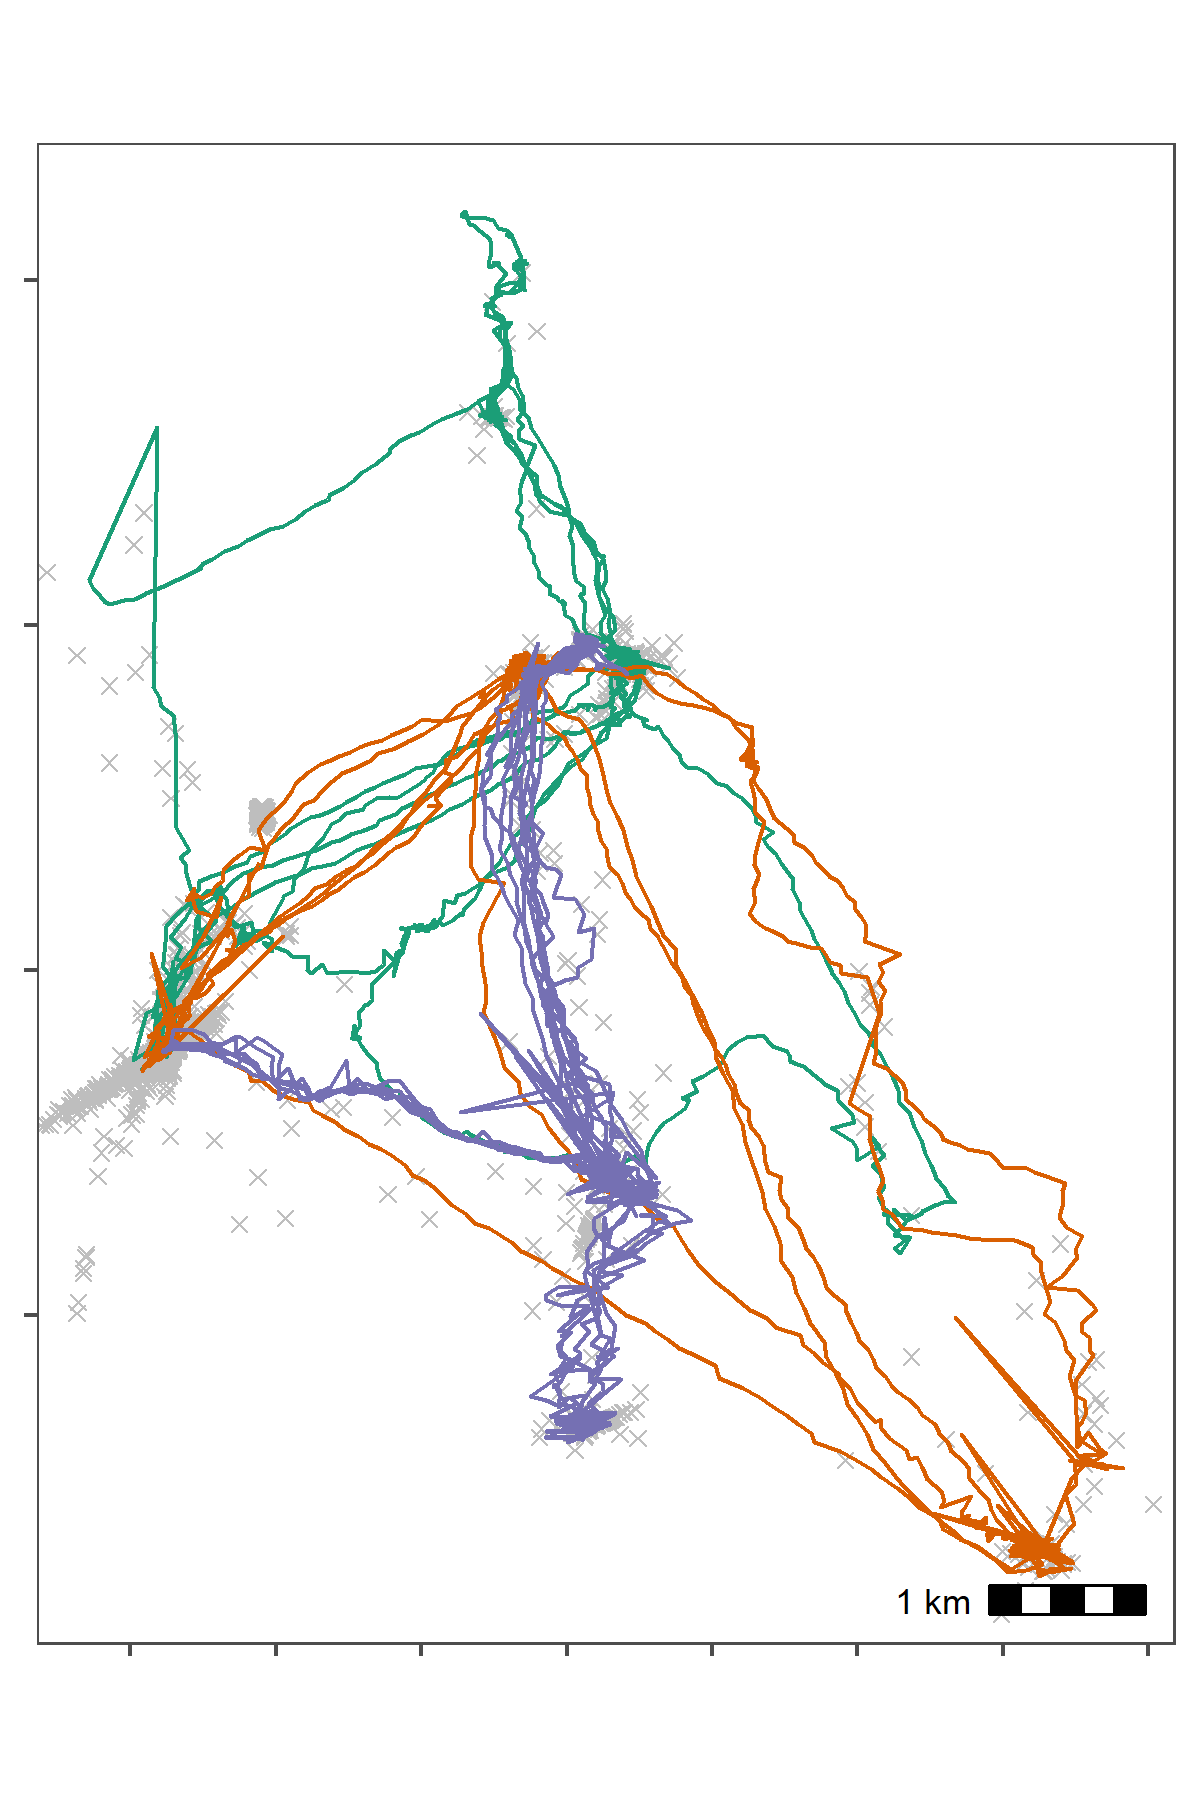
\includegraphics{figures/fig_bat_filter_cov.png}
\caption{Bat data filtered for large location errors, removing observations with standard deviation \(>\) 20. Grey crosses show data that were removed. Since the number of base stations used in the location process is a good indicator of error (Weiser et al. \protect\hyperlink{ref-weiser2016}{2016}), we also removed observations calculated using fewer than four base stations. Both steps used the function \texttt{atl\_filter\_covariates}.
This filtering reduced the data to an average of 10,447 positions per individual (78\% of the raw data on average). However, some point outliers remain.}
\end{figure}

\hypertarget{filter-by-speed}{%
\subsection{Filter by speed}\label{filter-by-speed}}

Some point outliers remain (Figure 2), and could be removed using a speed filter.

First we calculate speeds, using \texttt{atl\_get\_speed}. We must assign the speed output to a new column in the data.table, which has a special syntax which modifies in place, and is shown below. This syntax is a feature of the \texttt{data.table} package, not strictly of \texttt{atlastools} (Dowle and Srinivasan \protect\hyperlink{ref-dowle2020}{2020}).

\begin{Shaded}
\begin{Highlighting}[]
\CommentTok{\# get speeds as with SD, no reassignment required for columns}
\KeywordTok{invisible}\NormalTok{(}
  \KeywordTok{lapply}\NormalTok{(data\_split, }\ControlFlowTok{function}\NormalTok{(dt) \{}
    
    \CommentTok{\# first process time to seconds}
    \CommentTok{\# assign to a new column}
\NormalTok{    dt[, time }\OperatorTok{:}\ErrorTok{=}\StringTok{ }\KeywordTok{floor}\NormalTok{(TIME }\OperatorTok{/}\StringTok{ }\DecValTok{1000}\NormalTok{)]}
    
\NormalTok{    dt[, }\StringTok{\textasciigrave{}}\DataTypeTok{:=}\StringTok{\textasciigrave{}}\NormalTok{(}\DataTypeTok{speed\_in =} \KeywordTok{atl\_get\_speed}\NormalTok{(dt, }
                                       \DataTypeTok{x =} \StringTok{"X"}\NormalTok{, }\DataTypeTok{y =} \StringTok{"Y"}\NormalTok{, }
                                       \DataTypeTok{time =} \StringTok{"time"}\NormalTok{,}
                                       \DataTypeTok{type =} \StringTok{"in"}\NormalTok{),}
              \DataTypeTok{speed\_out =} \KeywordTok{atl\_get\_speed}\NormalTok{(dt, }
                                       \DataTypeTok{x =} \StringTok{"X"}\NormalTok{, }\DataTypeTok{y =} \StringTok{"Y"}\NormalTok{, }
                                       \DataTypeTok{time =} \StringTok{"time"}\NormalTok{,}
                                       \DataTypeTok{type =} \StringTok{"out"}\NormalTok{))]}
\NormalTok{  \})}
\NormalTok{)}
\end{Highlighting}
\end{Shaded}

Now filter for speeds \textgreater{} 20 m/s (around 70 km/h), passing the predicate (a statement return TRUE or FALSE) to \texttt{atl\_filter\_covariates}. First, we remove positions which have \texttt{NA} for their \texttt{speed\_in} (the first position) and their \texttt{speed\_out} (last position).

\begin{Shaded}
\begin{Highlighting}[]
\CommentTok{\# filter speeds}
\CommentTok{\# reassignment is required here}
\NormalTok{data\_split <{-}}\StringTok{ }\KeywordTok{lapply}\NormalTok{(data\_split, }\ControlFlowTok{function}\NormalTok{(dt) \{}
\NormalTok{  dt <{-}}\StringTok{ }\KeywordTok{na.omit}\NormalTok{(dt, }\DataTypeTok{cols =} \KeywordTok{c}\NormalTok{(}\StringTok{"speed\_in"}\NormalTok{, }\StringTok{"speed\_out"}\NormalTok{))}
  
\NormalTok{  dt <{-}}\StringTok{ }\KeywordTok{atl\_filter\_covariates}\NormalTok{(}\DataTypeTok{data =}\NormalTok{ dt,}
                              \DataTypeTok{filters =} \KeywordTok{c}\NormalTok{(}\StringTok{"speed\_in <= 20"}\NormalTok{,}
                                          \StringTok{"speed\_out <= 20"}\NormalTok{))}
\NormalTok{\})}
\end{Highlighting}
\end{Shaded}

\hypertarget{sanity-check-plot-speed-filtered-data}{%
\subsubsection{Sanity check: Plot speed filtered data}\label{sanity-check-plot-speed-filtered-data}}

The speed filtered data is now inspected for errors (Figure 3). The plot code is once again hidden.

\begin{figure}
\centering
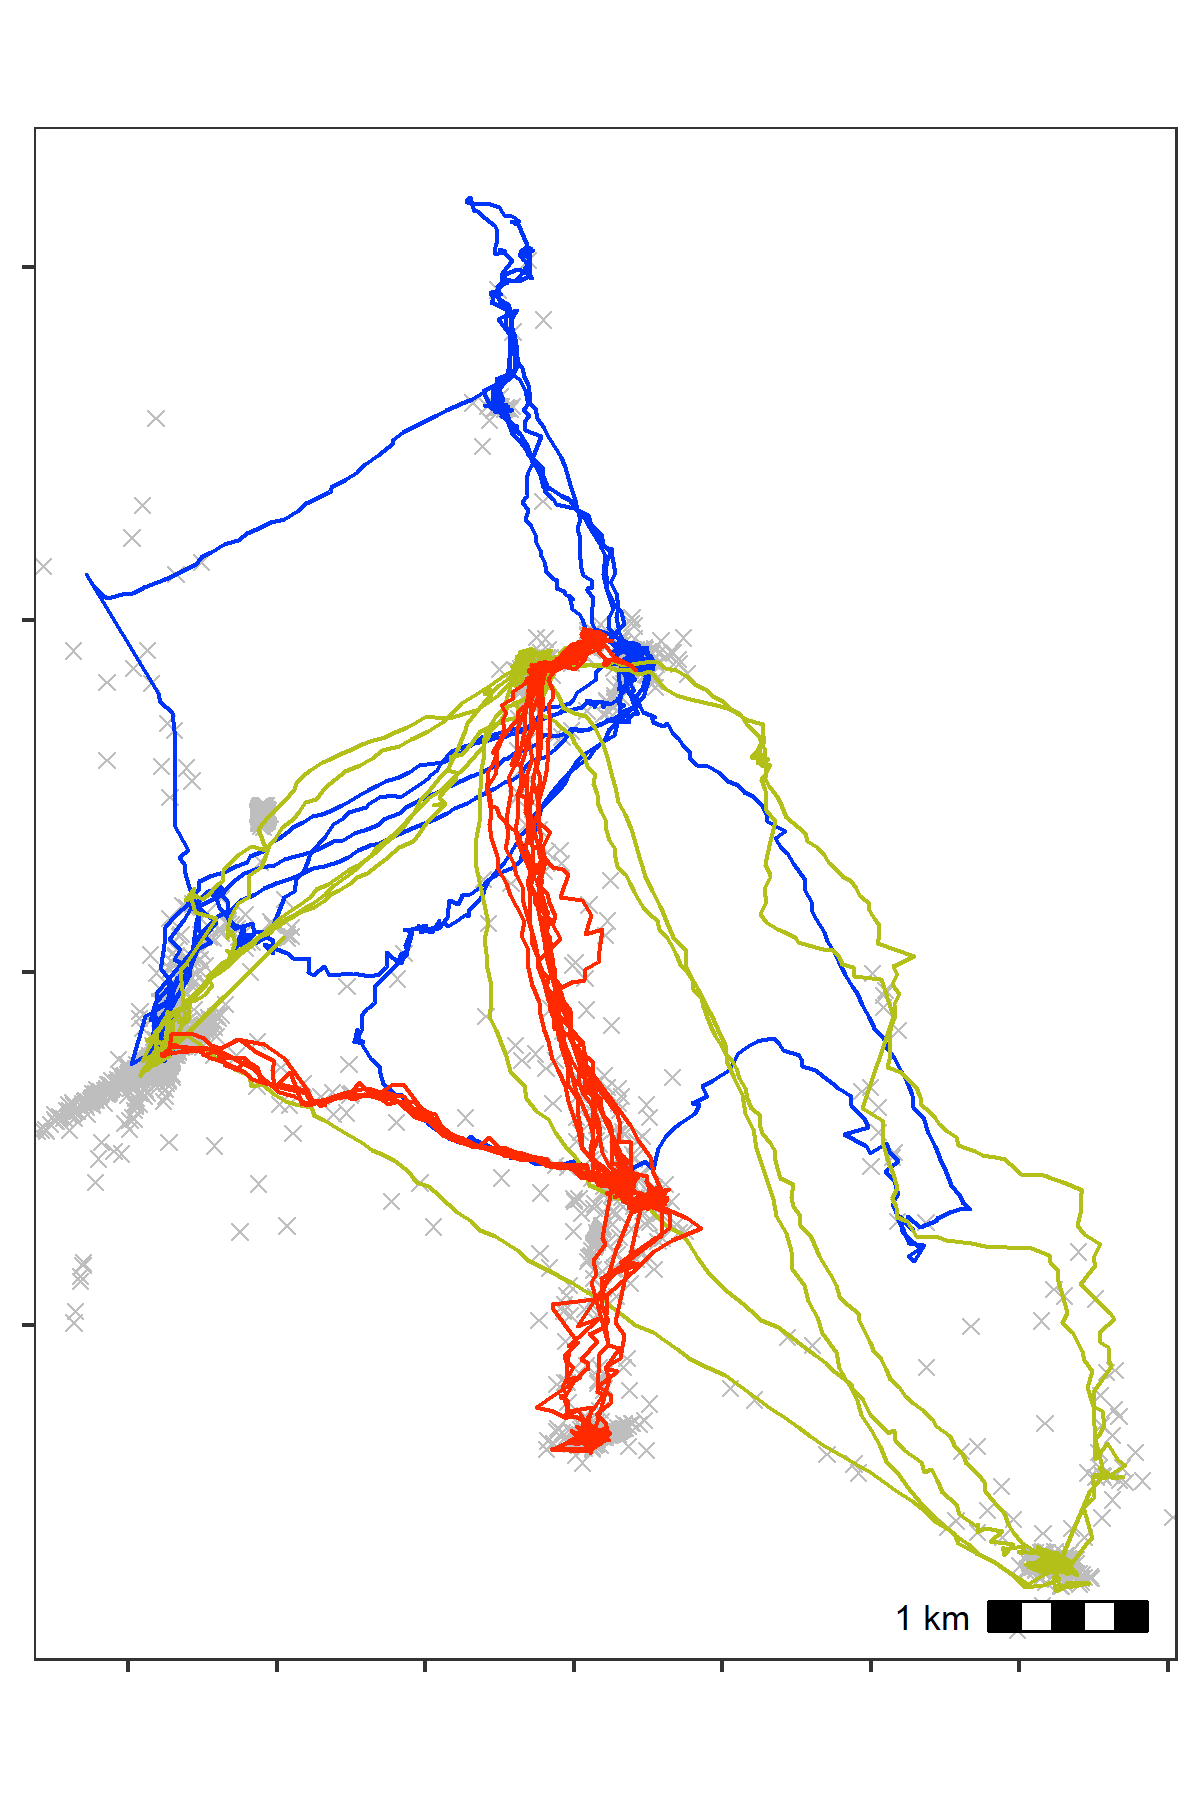
\includegraphics{figures/fig_bat_filter_speed.png}
\caption{Bat data with unrealistic speeds removed. Grey crosses show data that were removed. We calculated the incoming and outgoing speed of each position using \texttt{atl\_get\_speed}, and filtered out positions with speeds \textgreater{} 20 m/s using \texttt{atl\_filter\_covariates}, leaving 10,337 positions per individual on average (98\% from the previous step).}
\end{figure}

\hypertarget{median-smoothing}{%
\subsection{Median smoothing}\label{median-smoothing}}

The quality of this data (Figure 3) is relatively high, and a median smooth is not strictly necessary. We demonstrate the application of a 5 point median smooth to the data nonetheless.

Since the median smoothing function \texttt{atl\_median\_smooth} modifies in place, we first make a copy of the data, using \texttt{data.table}'s \texttt{copy} function.
No reassignment is required, in this case. The \texttt{lapply} function allows arguments to \texttt{atl\_median\_smooth} to be passed within \texttt{lapply} itself.

In this case, the same moving window \(K\) is applied to all individuals, but modifying this code to use the multivariate version \texttt{Map} allows different \(K\) to be used for different individuals. This is a programming matter, and is not covered here further.

\begin{Shaded}
\begin{Highlighting}[]
\CommentTok{\# since the function modifies in place, we shall make a copy}
\NormalTok{data\_smooth <{-}}\StringTok{ }\KeywordTok{copy}\NormalTok{(data\_split)}

\CommentTok{\# split the data again}
\NormalTok{data\_smooth <{-}}\StringTok{ }\KeywordTok{split}\NormalTok{(data\_smooth, }\DataTypeTok{by =} \StringTok{"TAG"}\NormalTok{)}
\end{Highlighting}
\end{Shaded}

\begin{Shaded}
\begin{Highlighting}[]
\CommentTok{\# apply the median smooth to each list element}
\CommentTok{\# no reassignment is required as THE FUNCTION MODIFIES IN PLACE!}
\KeywordTok{invisible}\NormalTok{(}
  
  \CommentTok{\# the function arguments to atl\_median\_smooth}
  \CommentTok{\# can be passed directly in lapply}
  
  \KeywordTok{lapply}\NormalTok{(}\DataTypeTok{X =}\NormalTok{ data\_smooth, }
         \DataTypeTok{FUN =}\NormalTok{ atl\_median\_smooth,}
         \DataTypeTok{time =} \StringTok{"time"}\NormalTok{, }\DataTypeTok{moving\_window =} \DecValTok{5}\NormalTok{)}
\NormalTok{)}
\end{Highlighting}
\end{Shaded}

\hypertarget{sanity-check-plot-smoothed-data}{%
\subsubsection{Sanity check: Plot smoothed data}\label{sanity-check-plot-smoothed-data}}

\begin{figure}
\centering
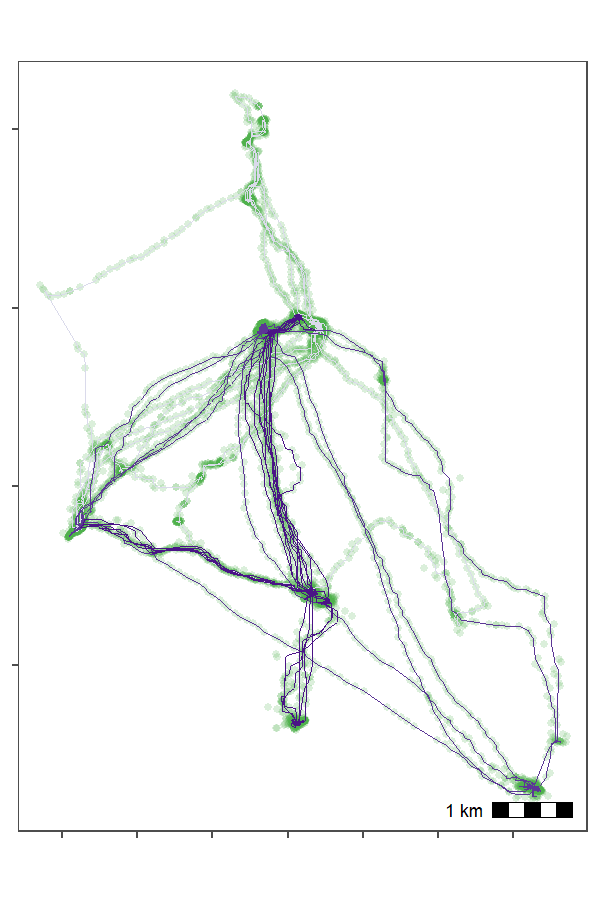
\includegraphics{figures/fig_bat_smooth.png}
\caption{Bat data after applying a median smooth with a moving window \(K\) = 5. Grey crosses show data prior to smoothing. The smoothing step did not discard any data.}
\end{figure}

\hypertarget{making-residence-patches}{%
\subsection{Making residence patches}\label{making-residence-patches}}

\hypertarget{calculating-residence-time}{%
\subsubsection{Calculating residence time}\label{calculating-residence-time}}

First, the data is put through the \texttt{recurse} package to get residence time (Bracis, Bildstein, and Mueller \protect\hyperlink{ref-bracis2018}{2018}).

\begin{Shaded}
\begin{Highlighting}[]
\CommentTok{\# load recurse}
\KeywordTok{library}\NormalTok{(recurse)}

\CommentTok{\# split the data}
\NormalTok{data\_smooth <{-}}\StringTok{ }\KeywordTok{split}\NormalTok{(data\_smooth, data\_smooth}\OperatorTok{$}\NormalTok{TAG)}
\end{Highlighting}
\end{Shaded}

We calculated residence time, but since bats may revisit the same features, we want to prevent confusion between frequent revisits and prolonged residence.

For this, we stop summing residence times within \(Z\) metres of a location if the animal exited the area for one hour or more. The value of \(Z\) (radius, in \texttt{recurse} parameter terms) was chosen as 50m.

This step is relatively complicated and is only required for individuals which frequently return to the same location, or pass over the same areas repeatedly, and for which revisits (cumulative time spent) may be confused for residence time in a single visit.

While a simpler implementation using total residence time divided by the number of revisits is also possible, this does assume that each revisit had the same residence time.

\begin{Shaded}
\begin{Highlighting}[]
\CommentTok{\# get residence times}

\NormalTok{data\_residence <{-}}\StringTok{ }\KeywordTok{lapply}\NormalTok{(data\_smooth, }\ControlFlowTok{function}\NormalTok{(dt) \{}
  \CommentTok{\# do basic recurse}
\NormalTok{  dt\_recurse <{-}}\StringTok{ }\KeywordTok{getRecursions}\NormalTok{(}
    \DataTypeTok{x =}\NormalTok{ dt[, }\KeywordTok{c}\NormalTok{(}\StringTok{"X"}\NormalTok{, }\StringTok{"Y"}\NormalTok{, }\StringTok{"time"}\NormalTok{, }\StringTok{"TAG"}\NormalTok{)],}
    \DataTypeTok{radius =} \DecValTok{50}\NormalTok{,}
    \DataTypeTok{timeunits =} \StringTok{"mins"}
\NormalTok{  )}
  
  \CommentTok{\# get revisit stats}
\NormalTok{  dt\_recurse <{-}}\StringTok{ }\KeywordTok{setDT}\NormalTok{(}
\NormalTok{    dt\_recurse[[}\StringTok{"revisitStats"}\NormalTok{]]}
\NormalTok{  )}
  
  \CommentTok{\# count long absences from the area}
\NormalTok{  dt\_recurse[, timeSinceLastVisit }\OperatorTok{:}\ErrorTok{=}
\StringTok{          }\KeywordTok{ifelse}\NormalTok{(}\KeywordTok{is.na}\NormalTok{(timeSinceLastVisit), }\OperatorTok{{-}}\OtherTok{Inf}\NormalTok{, timeSinceLastVisit)]}
\NormalTok{  dt\_recurse[, longAbsenceCounter }\OperatorTok{:}\ErrorTok{=}\StringTok{ }\KeywordTok{cumsum}\NormalTok{(timeSinceLastVisit }\OperatorTok{>}\StringTok{ }\DecValTok{60}\NormalTok{),}
\NormalTok{             by =}\StringTok{ }\NormalTok{.(coordIdx)}
\NormalTok{             ]}
  \CommentTok{\# get data before the first long absence of 60 mins}
\NormalTok{  dt\_recurse <{-}}\StringTok{ }\NormalTok{dt\_recurse[longAbsenceCounter }\OperatorTok{<}\StringTok{ }\DecValTok{1}\NormalTok{, ]}
  
\NormalTok{  dt\_recurse <{-}}\StringTok{ }\NormalTok{dt\_recurse[, }\KeywordTok{list}\NormalTok{(}
    \DataTypeTok{resTime =} \KeywordTok{sum}\NormalTok{(timeInside),}
    \DataTypeTok{fpt =} \KeywordTok{first}\NormalTok{(timeInside),}
    \DataTypeTok{revisits =} \KeywordTok{max}\NormalTok{(visitIdx)}
\NormalTok{  ),}
\NormalTok{  by =}\StringTok{ }\NormalTok{.(coordIdx, x, y)}
\NormalTok{  ]}
  
  \CommentTok{\# prepare and merge existing data with recursion data}
\NormalTok{  dt[, coordIdx }\OperatorTok{:}\ErrorTok{=}\StringTok{ }\KeywordTok{seq}\NormalTok{(}\KeywordTok{nrow}\NormalTok{(dt))]}
  
\NormalTok{  dt <{-}}\StringTok{ }\KeywordTok{merge}\NormalTok{(dt, }
\NormalTok{              dt\_recurse[, }\KeywordTok{c}\NormalTok{(}\StringTok{"coordIdx"}\NormalTok{, }\StringTok{"resTime"}\NormalTok{)], }
              \DataTypeTok{by =} \KeywordTok{c}\NormalTok{(}\StringTok{"coordIdx"}\NormalTok{))}
  
  \KeywordTok{setorderv}\NormalTok{(dt, }\StringTok{"time"}\NormalTok{)}
\NormalTok{\})}
\end{Highlighting}
\end{Shaded}

We bind the data together and assign a human readable timestamp column.

\begin{Shaded}
\begin{Highlighting}[]
\CommentTok{\# bind the list}
\NormalTok{data\_residence <{-}}\StringTok{ }\KeywordTok{rbindlist}\NormalTok{(data\_residence)}

\CommentTok{\# get time as human readable}
\NormalTok{data\_residence[, ts }\OperatorTok{:}\ErrorTok{=}\StringTok{ }\KeywordTok{as.POSIXct}\NormalTok{(time, }\DataTypeTok{origin =} \StringTok{"1970{-}01{-}01"}\NormalTok{)]}
\end{Highlighting}
\end{Shaded}

\hypertarget{constructing-residence-patches}{%
\subsubsection{Constructing residence patches}\label{constructing-residence-patches}}

Some preparation is required. First, the function requires columns \texttt{x}, \texttt{y},
\texttt{time}, and \texttt{id}, which we assign using the \texttt{data.table} syntax.
Then we subset the data to only work with positions where the individual had a residence time of more than 5 minutes.

\begin{Shaded}
\begin{Highlighting}[]
\CommentTok{\# add an id column}
\NormalTok{data\_residence[, }\StringTok{\textasciigrave{}}\DataTypeTok{:=}\StringTok{\textasciigrave{}}\NormalTok{(}\DataTypeTok{id =}\NormalTok{ TAG,}
                      \DataTypeTok{x =}\NormalTok{ X, }\DataTypeTok{y =}\NormalTok{ Y)]}

\CommentTok{\# filter for residence time > 5 minutes}
\NormalTok{data\_residence <{-}}\StringTok{ }\NormalTok{data\_residence[resTime }\OperatorTok{>}\StringTok{ }\DecValTok{5}\NormalTok{, ]}

\CommentTok{\# split the data}
\NormalTok{data\_residence <{-}}\StringTok{ }\KeywordTok{split}\NormalTok{(data\_residence, data\_residence}\OperatorTok{$}\NormalTok{TAG)}
\end{Highlighting}
\end{Shaded}

We apply the residence patch method, using the default argument values (\texttt{lim\_spat\_indep\ =\ 100} (metres), \texttt{lim\_time\_indep\ =\ 30} (minutes), and \texttt{min\_fixes\ =\ 3}). We change the \texttt{buffer\_radius} to 25 metres (twice the buffer radius is used, so points must be separated by 50m to be independent bouts).

\begin{Shaded}
\begin{Highlighting}[]
\CommentTok{\# segment into residence patches}
\NormalTok{data\_patches <{-}}\StringTok{ }\KeywordTok{lapply}\NormalTok{(data\_residence, atl\_res\_patch,}
                       \DataTypeTok{buffer\_radius =} \DecValTok{25}\NormalTok{)}
\end{Highlighting}
\end{Shaded}

\hypertarget{getting-residence-patch-data}{%
\subsubsection{Getting residence patch data}\label{getting-residence-patch-data}}

We extract the residence patch data as spatial \texttt{sf-MULTIPOLYGON} objects.
These are returned as a list and must be converted into a single \texttt{sf} object.
These objects and the raw movement data are shown in Figure 5.

\begin{Shaded}
\begin{Highlighting}[]
\CommentTok{\# get data spatials}
\NormalTok{data\_spatials <{-}}\StringTok{ }\KeywordTok{lapply}\NormalTok{(data\_patches, atl\_patch\_summary,}
                        \DataTypeTok{which\_data =} \StringTok{"spatial"}\NormalTok{,}
                        \DataTypeTok{buffer\_radius =} \DecValTok{25}\NormalTok{)}

\CommentTok{\# bind list}
\NormalTok{data\_spatials <{-}}\StringTok{ }\KeywordTok{rbindlist}\NormalTok{(data\_spatials)}

\CommentTok{\# convert to sf}
\KeywordTok{library}\NormalTok{(sf)}
\NormalTok{data\_spatials <{-}}\StringTok{ }\KeywordTok{st\_sf}\NormalTok{(data\_spatials, }\DataTypeTok{sf\_column\_name =} \StringTok{"polygons"}\NormalTok{)}

\CommentTok{\# assign a crs}
\KeywordTok{st\_crs}\NormalTok{(data\_spatials) <{-}}\StringTok{ }\KeywordTok{st\_crs}\NormalTok{(}\DecValTok{2039}\NormalTok{)}
\end{Highlighting}
\end{Shaded}

\hypertarget{write-patch-spatial-representations}{%
\subsubsection{Write patch spatial representations}\label{write-patch-spatial-representations}}

\begin{Shaded}
\begin{Highlighting}[]
\KeywordTok{st\_write}\NormalTok{(data\_spatials,}
         \DataTypeTok{dsn =} \StringTok{"data/data\_bat\_residence\_patches.gpkg"}\NormalTok{)}
\end{Highlighting}
\end{Shaded}

Write cleaned bat data.

\begin{Shaded}
\begin{Highlighting}[]
\NormalTok{data\_clean <{-}}\StringTok{ }\KeywordTok{fwrite}\NormalTok{(}\KeywordTok{rbindlist}\NormalTok{(data\_smooth),}
                     \DataTypeTok{file =} \StringTok{"data/data\_bat\_smooth.csv"}\NormalTok{)}
\end{Highlighting}
\end{Shaded}

Write patch summary.

\begin{Shaded}
\begin{Highlighting}[]
\CommentTok{\# get summary}
\NormalTok{patch\_summary <{-}}\StringTok{ }\KeywordTok{lapply}\NormalTok{(data\_patches, atl\_patch\_summary)}

\CommentTok{\# bind summary}
\NormalTok{patch\_summary <{-}}\StringTok{ }\KeywordTok{rbindlist}\NormalTok{(patch\_summary)}

\CommentTok{\# write}
\KeywordTok{fwrite}\NormalTok{(patch\_summary,}
       \StringTok{"data/data\_bat\_patch\_summary.csv"}\NormalTok{)}
\end{Highlighting}
\end{Shaded}

\begin{figure}
\centering
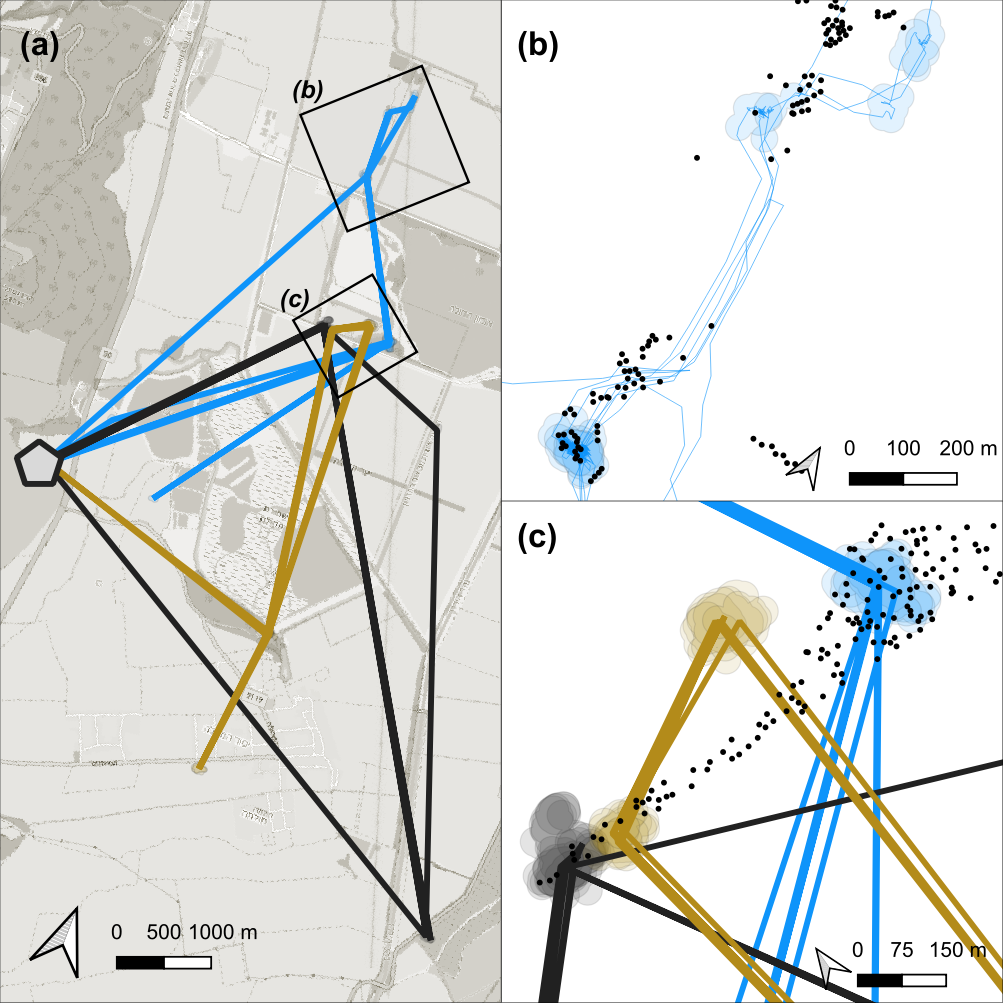
\includegraphics{figures/fig_08_bats.png}
\caption{A visual examination of plots of the bats' residence patches and linear approximations of paths between them showed that though all three bats roosted at the same site, they used distinct areas of the study site over the three nights \textbf{(a)}.
Bats tended to be resident near fruit trees, which are their main food source, travelling repeatedly between previously visited areas \textbf{(b, c)}.
However, bats also appeared to spend some time at locations where no fruit trees were recorded, prompting questions about their use of other food sources \textbf{(b, c)}.
When bats did occur close together, their residence patches barely overlapped, and their paths to and from the broad area of co-occurrence were not similar \textbf{(c)}.
Constructing residence patches for multiple individuals over multiple activity periods suggests interesting dynamics of within- and between-individual overlap \textbf{(b, c)}.}
\end{figure}

\hypertarget{references}{%
\section{References}\label{references}}

\hypertarget{refs}{}
\begin{cslreferences}
\leavevmode\hypertarget{ref-barraquand2008}{}%
Barraquand, Frédéric, and Simon Benhamou. 2008. ``Animal Movements in Heterogeneous Landscapes: Identifying Profitable Places and Homogeneous Movement Bouts.'' \emph{Ecology} 89 (12): 3336--48. \url{https://doi.org/10.1890/08-0162.1}.

\leavevmode\hypertarget{ref-bijleveld2016}{}%
Bijleveld, Allert Imre, Robert B MacCurdy, Ying-Chi Chan, Emma Penning, Richard M. Gabrielson, John Cluderay, Erik L. Spaulding, et al. 2016. ``Understanding Spatial Distributions: Negative Density-Dependence in Prey Causes Predators to Trade-Off Prey Quantity with Quality.'' \emph{Proceedings of the Royal Society B: Biological Sciences} 283 (1828): 20151557. \url{https://doi.org/10.1098/rspb.2015.1557}.

\leavevmode\hypertarget{ref-bracis2018}{}%
Bracis, Chloe, Keith L. Bildstein, and Thomas Mueller. 2018. ``Revisitation Analysis Uncovers Spatio-Temporal Patterns in Animal Movement Data.'' \emph{Ecography} 41 (11): 1801--11. \url{https://doi.org/10.1111/ecog.03618}.

\leavevmode\hypertarget{ref-dowle2020}{}%
Dowle, Matt, and Arun Srinivasan. 2020. \emph{Data.Table: Extension of `data.Frame`}. Manual.

\leavevmode\hypertarget{ref-gupte2020a}{}%
Gupte, Pratik Rajan. 2020. ``Atlastools: Pre-Processing Tools for High Frequency Tracking Data.'' Zenodo. \url{https://doi.org/10.5281/ZENODO.4033154}.

\leavevmode\hypertarget{ref-oudman2018}{}%
Oudman, Thomas, Theunis Piersma, Mohamed V. Ahmedou Salem, Marieke E. Feis, Anne Dekinga, Sander Holthuijsen, Job ten Horn, Jan A. van Gils, and Allert I. Bijleveld. 2018. ``Resource Landscapes Explain Contrasting Patterns of Aggregation and Site Fidelity by Red Knots at Two Wintering Sites.'' \emph{Movement Ecology} 6 (1): 24--24. \url{https://doi.org/10.1186/s40462-018-0142-4}.

\leavevmode\hypertarget{ref-shohami2020}{}%
Shohami, David, and Ran Nathan. 2020. ``Cognitive Map-Based Navigation in Wild Bats Revealed by a New High-Throughput Tracking System.'' Dryad. \url{https://doi.org/10.5061/DRYAD.G4F4QRFN2}.

\leavevmode\hypertarget{ref-toledo2020}{}%
Toledo, Sivan, David Shohami, Ingo Schiffner, Emmanuel Lourie, Yotam Orchan, Yoav Bartan, and Ran Nathan. 2020. ``Cognitive MapBased Navigation in Wild Bats Revealed by a New High-Throughput Tracking System.'' \emph{Science} 369 (6500): 188--93. \url{https://doi.org/10.1126/science.aax6904}.

\leavevmode\hypertarget{ref-weiser2016}{}%
Weiser, Adi Weller, Yotam Orchan, Ran Nathan, Motti Charter, Anthony J. Weiss, and Sivan Toledo. 2016. ``Characterizing the Accuracy of a Self-Synchronized Reverse-GPS Wildlife Localization System.'' In \emph{2016 15th ACM/IEEE International Conference on Information Processing in Sensor Networks (IPSN)}, 1--12. \url{https://doi.org/10.1109/IPSN.2016.7460662}.
\end{cslreferences}

\end{document}
